\section{Förstärkare}
\textbf{HAREC a.\ref{HAREC.a.3.4}\label{myHAREC.a.3.4}}
\index{förstärkare}
\index{amplifier}
\index{blandning}
\index{mixing}

\subsection{Allmänt}

\begin{figure}
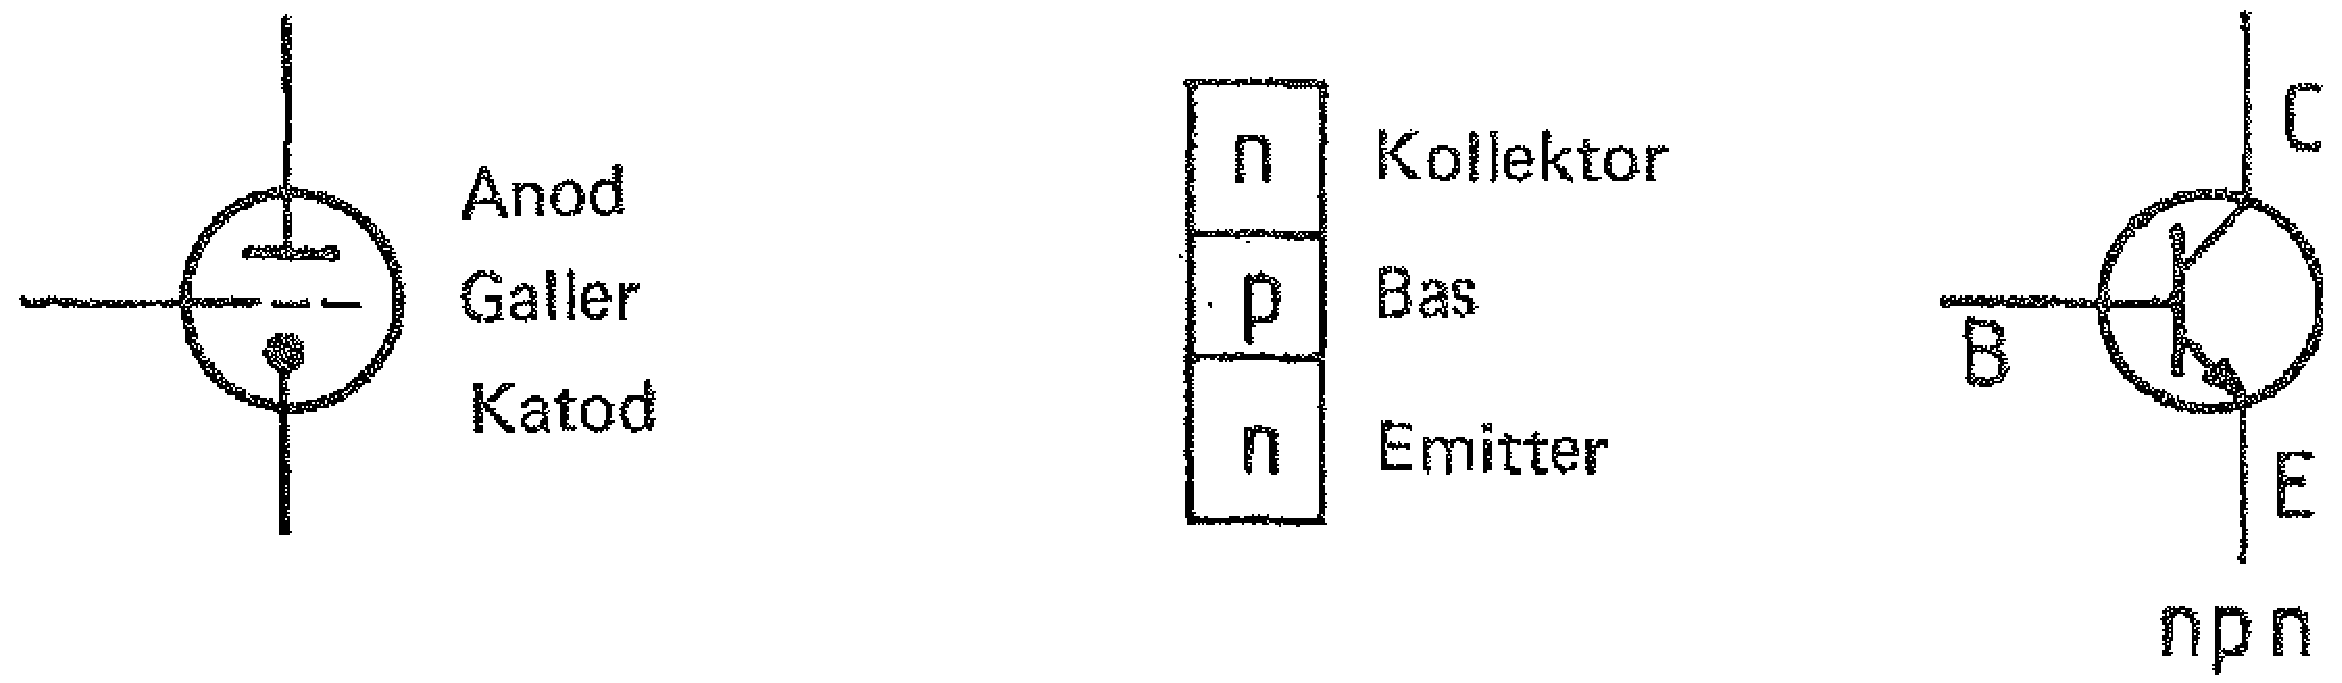
\includegraphics[width=\textwidth]{images/cropped_pdfs/bild_2_3-40.pdf}
\caption{Från elektronrör till transistor}
\label{fig:BildII3-40}
\end{figure}

Elektronrör och transistorer, se bild \ref{fig:BildII3-40}, är de
\emph{aktiva komponenter} (eng. \emph{active components}) som används i
oräkneliga elektroniska kopplingar för alstring av signaler, för
\emph{förstärkning} (eng. \emph{amplifier}) och \emph{blandning} (eng.
\emph{mixing}) av signaler, för multiplicering av signalfrekvenser etc.

Transistorn presenteras i avsnitt \ref{transistorn} och elektronröret i avsnitt \ref{elektronrör}.

Först förekom endast elektronrör.
Dessa har emellertid nästan helt ersatts av transistorer.
Elektronrör används dock fortfarande i viss mån, då främst i effektförstärkare
för sändare.
Det finns därför skäl att här behandla såväl elektronrör som transistorer.

\subsection{Huvudegenskaper hos förstärkare}
\subsubsection{LF- och HF-förstärkare}
\textbf{HAREC a.\ref{HAREC.a.3.4.1}, a.\ref{HAREC.a.3.4.2}, a.\ref{HAREC.a.3.4.3}\label{myHAREC.a.3.4.1}\label{myHAREC.a.3.4.2}\label{myHAREC.a.3.4.3}}

\begin{figure}
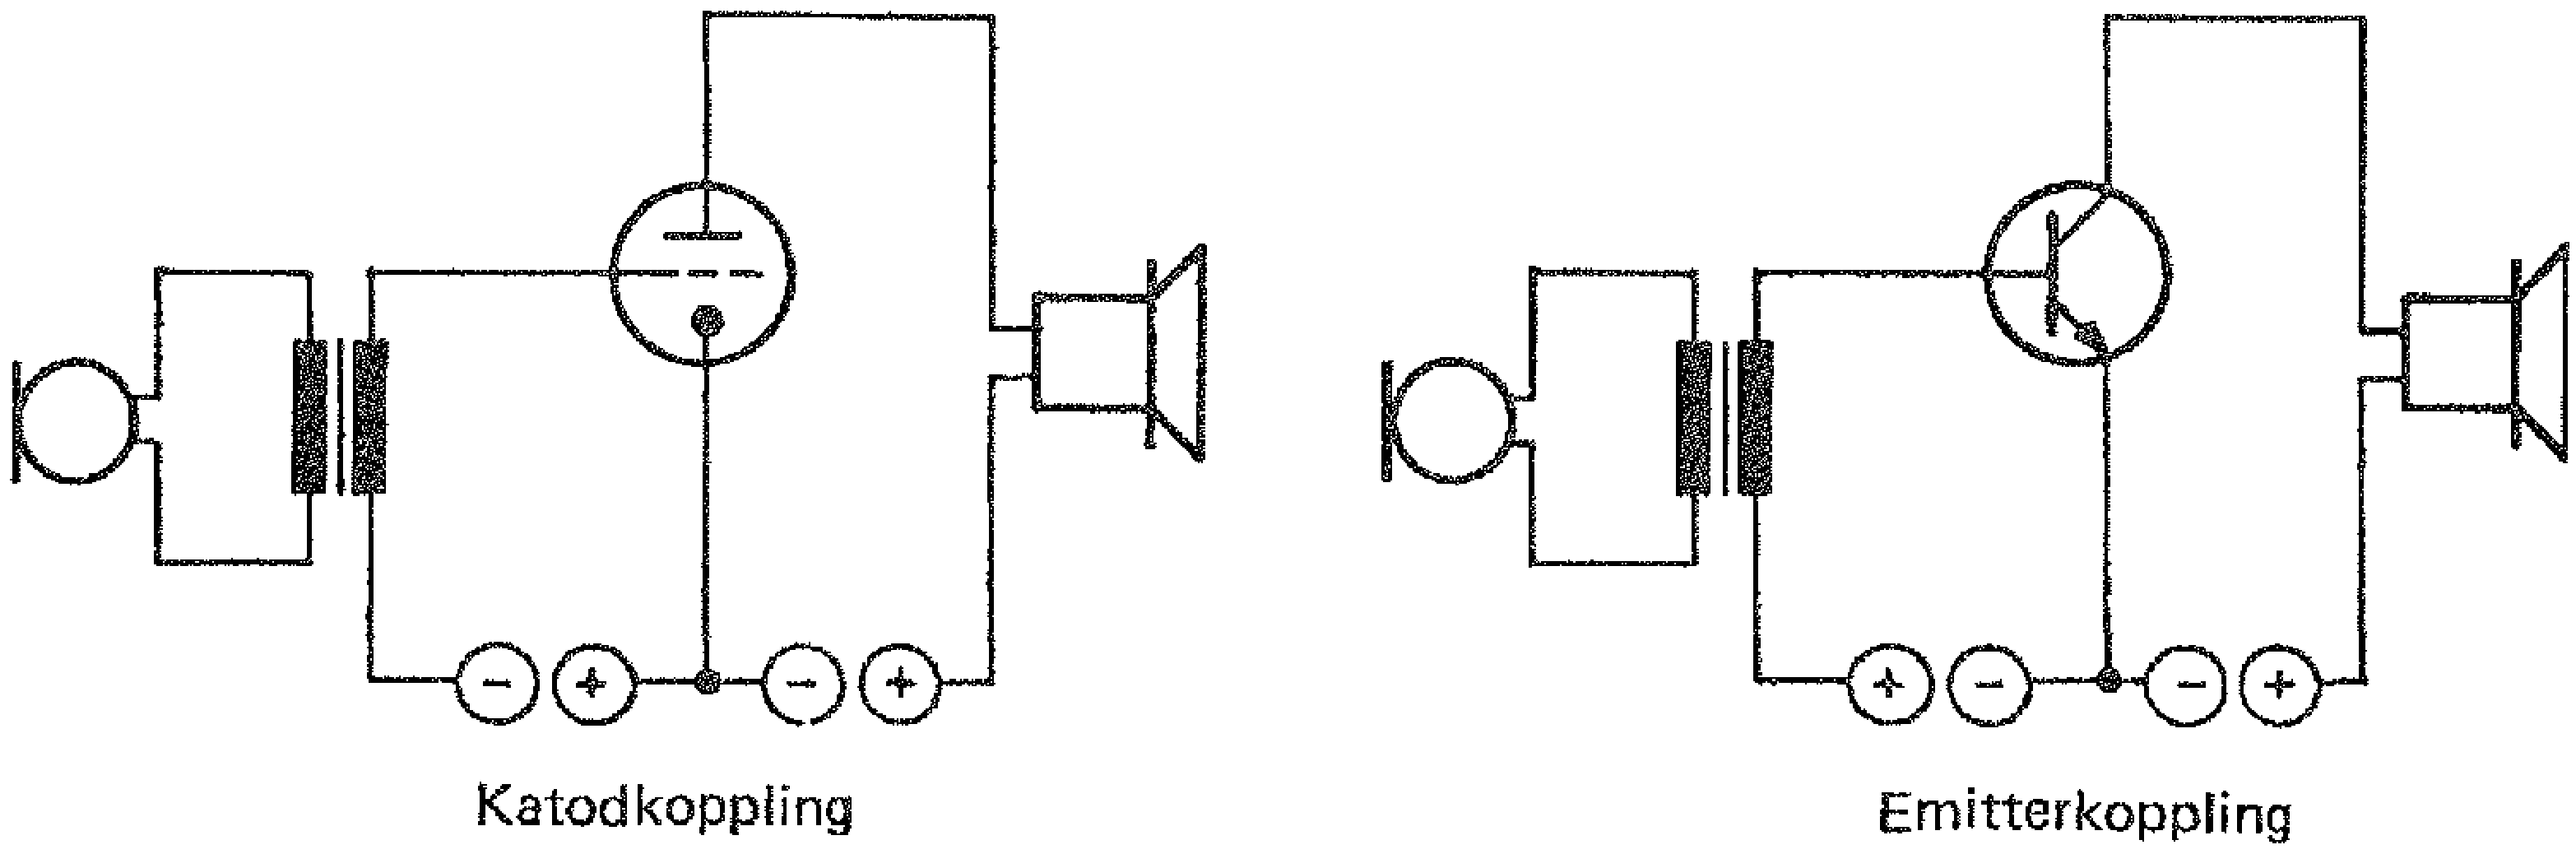
\includegraphics[width=\textwidth]{images/cropped_pdfs/bild_2_3-41.pdf}
\caption{Principen för förstärkare med elektronrör respektive transistor}
\label{fig:BildII3-41}
\end{figure}

Bild \ref{fig:BildII3-41} visar principen för förstärkare med både elektronrör
och transistor.

\index{LF-förstärkare}
\index{förstärkare!LF}
Med \emph{LF-förstärkare} menas förstärkare som arbetar med signaler i
det lägre frekvensområdet, typiskt upp till ca 100~kHz.
LF-förstärkare är mycket vanliga såväl i mottagare som sändare.
Utöver de aktiva komponenterna (transistorer, elektronrör) är kondensatorer
och resistorer de viktigaste passiva.

\index{HF-förstärkare}
\index{förstärkare!HF}
Med \emph{HF-förstärkare} menas förstärkare som arbetar med signaler
med högre frekvenser än dem i LF-området.
Även HF-förstärkare är mycket vanliga såväl i mottagare som sändare.
De används till exempel i mottagarnas ingångs- och mellanfrekvenssteg, liksom i
sändarnas oscillatorer, signalberedningssteg och slutsteg.
Utöver de komponenter, som även finns i LF-förstärkare, används kombinationer
av frekvensberoende komponenter såsom induktorer och kondensatorer.

\paragraph{Förstärkning}
\index{förstärkning}
\index{förstärkare!förstärkning}
\index{gain}

Med \emph{förstärkning} (eng. \emph{gain}) avses här kvoten av amplituden i
utgående och inkommande signal, varvid frekvensgången har inverkan.

\paragraph{Frekvensgång}
\index{frekvensgång}
Förstärkare arbetar endast inom ett visst frekvensområde, vilket kan
skilja från fall till fall.

\paragraph{Bandbredd}
\index{bandbredd}
\index{förstärkare!bandbredd}
\index{bandwidth|see {bandbredd}}

Det frekvensområde där förstärkaren arbetar med fulla data kallas
\emph{bandbredd} (eng. \emph{bandwidth}).
Bandgränserna uttrycks som en nedre och övre gränsfrekvens, där signalnivån
avviker från ett givet värde, vanligen med högst 3~dB.

För LF-förstärkare för amatörradiobruk är kravet på bandbredd litet; inom ett
band av 300~Hz till 3~kHz uppnås godtagbar återgivningskvalitet för tal.
Bandbredden bestäms främst av kondensatorer i kretsen avsedda för överföring
och avkoppling.

HF-förstärkare används för signaler med hög frekvens, typiskt 100~kHz och
däröver.
Det finns så kallade bredbandiga förstärkare för ett stort frekvensområde, men
även avstämda förstärkare för smala frekvensband.

\subsection{Grundkopplingar för förstärkarsteg}
\textbf{HAREC a.\ref{HAREC.a.2.6.4.1}, a.\ref{HAREC.a.2.6.4.2}, a.\ref{HAREC.a.2.6.4.3}, a.\ref{HAREC.a.2.6.4.4}\label{myHAREC.a.2.6.4.1}\label{myHAREC.a.2.6.4.2}\label{myHAREC.a.2.6.4.3}\label{myHAREC.a.2.6.4.4}}

\begin{figure}
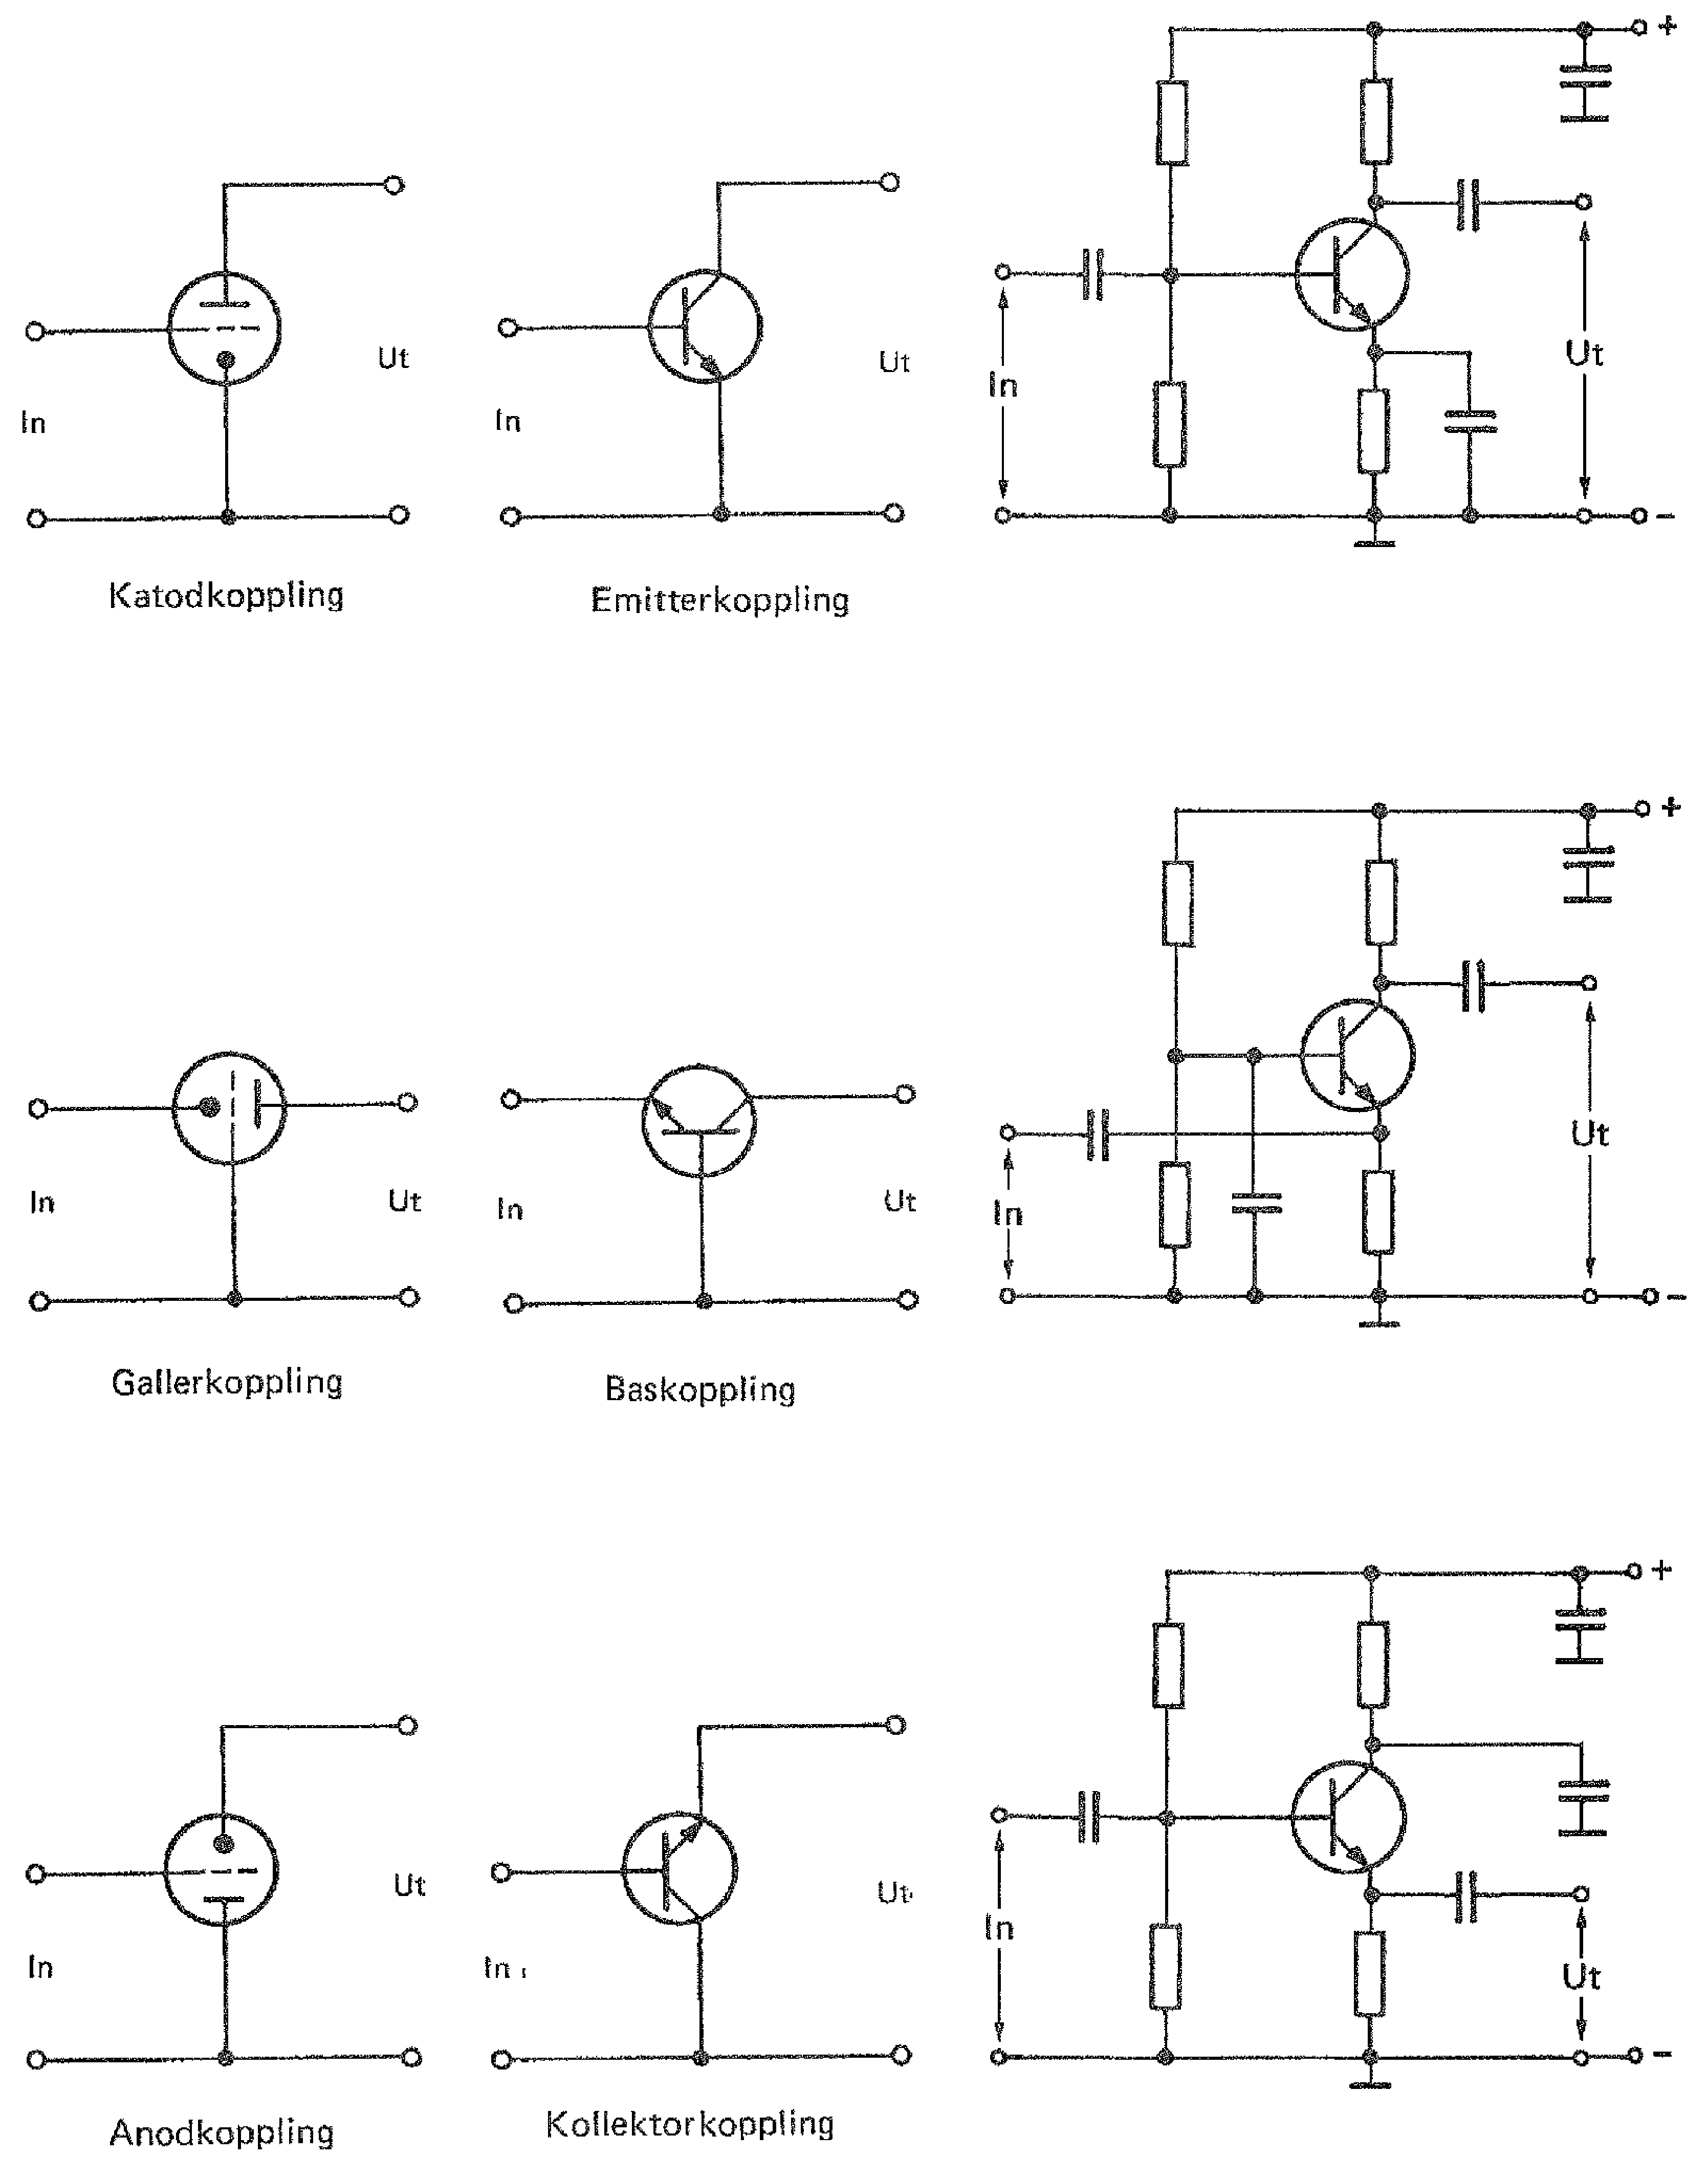
\includegraphics[width=\textwidth]{images/cropped_pdfs/bild_2_3-42.pdf}
\caption{Grundkopplingar för elektronrör och NPN-transistor}
\label{fig:BildII3-42}
\end{figure}

I det föregående har redan visats att en av polerna i ingången respektive
utgången i en förstärkare är gemensam.
I bild \ref{fig:BildII3-42} är rörförstärkarens katod den gemensamma
polen -- därav namnet katodkoppling.
På liknande sätt är NPN-transistorns emitter gemensam
-- därav namnet emitterkoppling.

På ett liknande sätt kan någon annan pol vara gemensam.
Man får då i stället en baskoppling eller kollektorkoppling.

Beroende av kopplingssätt fås olika egenskaper.
På nästa sida visas tre olika grundkopplingar för ett elektronrör (triod)
respektive en NPN-transistor.

I praktiken känns en grundkoppling igen på vilken elektrod som är
avkopplad till 0-potential över en kondensator.

\index{emitterkoppling}
\index{förstärkare!emitterkoppling}
\emph{Emitterkoppling} används för LF och HF när hög förstärkning eftersträvas.
Eftersom effektförstärkningen är produkten av spännings- och
strömförstärkningen, så fås en effektförstärkning av mellan 200 till 50000
gånger.
Nackdelen med denna koppling är den ibland låga ingångsimpedansen och den
relativt låga gränsfrekvensen.

\index{baskoppling}
\index{förstärkare!baskoppling}
\emph{Baskoppling} använd som HF-förstärkare på grund av sin höga
gränsfrekvens och goda isolation mellan in- och utgång.

\index{kollektorkoppling}
\index{förstärkare!kollektorkoppling}
\emph{Kollektorkoppling} används när hög ingångsimpedans och
utgångsimpedans önskas.
Denna koppling har emellertid ingenspänningsförstärkning, men kan användas för
så kallad impedansomvandling.

\begin{table*}[!h]
\caption{Grundkopplingarnas typiska egenskaper vid NPN-transistor}
  \begin{tabular}{p{0.20\textwidth}|p{0.30\textwidth}|p{0.20\textwidth}|p{0.25\textwidth}}
    \bf Egenskap & \bf Emitterkoppling & \bf Baskoppling & \bf Kollektor\-koppling \\
    \(Z_{in}\) & medel \quad 1 k\(\Omega\) & liten \quad 50 \(\Omega\) & stor \quad 100 k\(\Omega\) \\
    \(Z_{ut}\) & medel \quad 10 k\(\Omega\) & stor \quad 100 k\(\Omega\) & liten \quad 50 k\(\Omega\) \\
    Förstärkning & & & \\
    \quad Ström- & stor \quad 100 ggr & <1 \quad 0,9 ggr & stor \quad 100 ggr \\
    \quad Spänning- & stor \quad 100 ggr & stor \quad 100 ggr & <1 \quad 0,99 ggr \\
    \quad Effekt- & mycket stor 10000 ggr & stor \quad 100 ggr & stor \quad 100 ggr \\
    Fasläge & motfas \quad 180\degree & medfas \quad 0\degree & medfas 0\degree \\
  \end{tabular}
\end{table*}


%%


\subsection{Stabilisering av arbetspunkten}

För att en förstärkare ska kunna arbeta på avsett sätt måste
arbetspunkten, det vill säga arbetsströmmens vilovärde ställas rätt.

Det gör man genom att placera en förspänning över den styrande
elektroden i elektronröret eller transistorn i fråga.

I en katodkopplad rörförstärkare innebär det att styrgallret ska
ges en viss negativ spänning i förhållande till katoden.
Det kan man göra till exempel med en separat spänningskälla eller vanligare med
en avkopplad resistor mellan katod och minuspolen (jord).

I en emitterkopplad transistorförstärkare innebär det att basen ska
ges en viss positiv spänning i förhållande till emittern.
Det kan man göra till exempel med en separat spänningskälla eller vanligare med
en avkopplad resistor mellan emittern och minuspolen samt en resistiv
spänningsdelare mellan plus- och minuspolen.

\subsection{Klass A-, B- och C-förstärkare}
\textbf{HAREC a.\ref{HAREC.a.3.4.4}\label{myHAREC.a.3.4.4}}

\subsubsection{Arbetspunkt}
\index{arbetspunkt}
\index{distorsion}

\emph{Arbetspunkten} för förstärkare väljs olika, beroende på önskat arbetssätt.
En olämpligt vald arbetspunkt resulterar i förvrängning av utsignalens form i
förhållande till insignalens form, så kallad \emph{distorsion}.
Distorsion uppstår även vid överstyrning, det vill säga när insignalens
amplitud är för stor för att kunna återges med oförändrad form, även om
arbetspunkten är rätt vald.

Med avseende på arbetspunktens läge klassas därför förstärkare på sätt
som framgår av följande diagram för transistorer eller elektronrör.
En emitterjordad NPN-transistor får anses mest motsvara
elektronrörskopplingen här nedan.
Anodströmmen \(I_a\) motsvaras då närmast av kollektorströmmen
\(I_C\) och styrgallerspänningen \(U_{gi}\) av spänningen
\(U_{BE}\).
Den stora skillnaden är att styrgallerspänningen i dessa
fall alltid är negativ medan bas/emitterspänningen är positiv.
Styrspänningens relativa läge (arbetspunkten) mellan olika
arbetsklasser är emellertid lika.

\begin{wrapfigure}[37]{R}{0.3\textwidth}
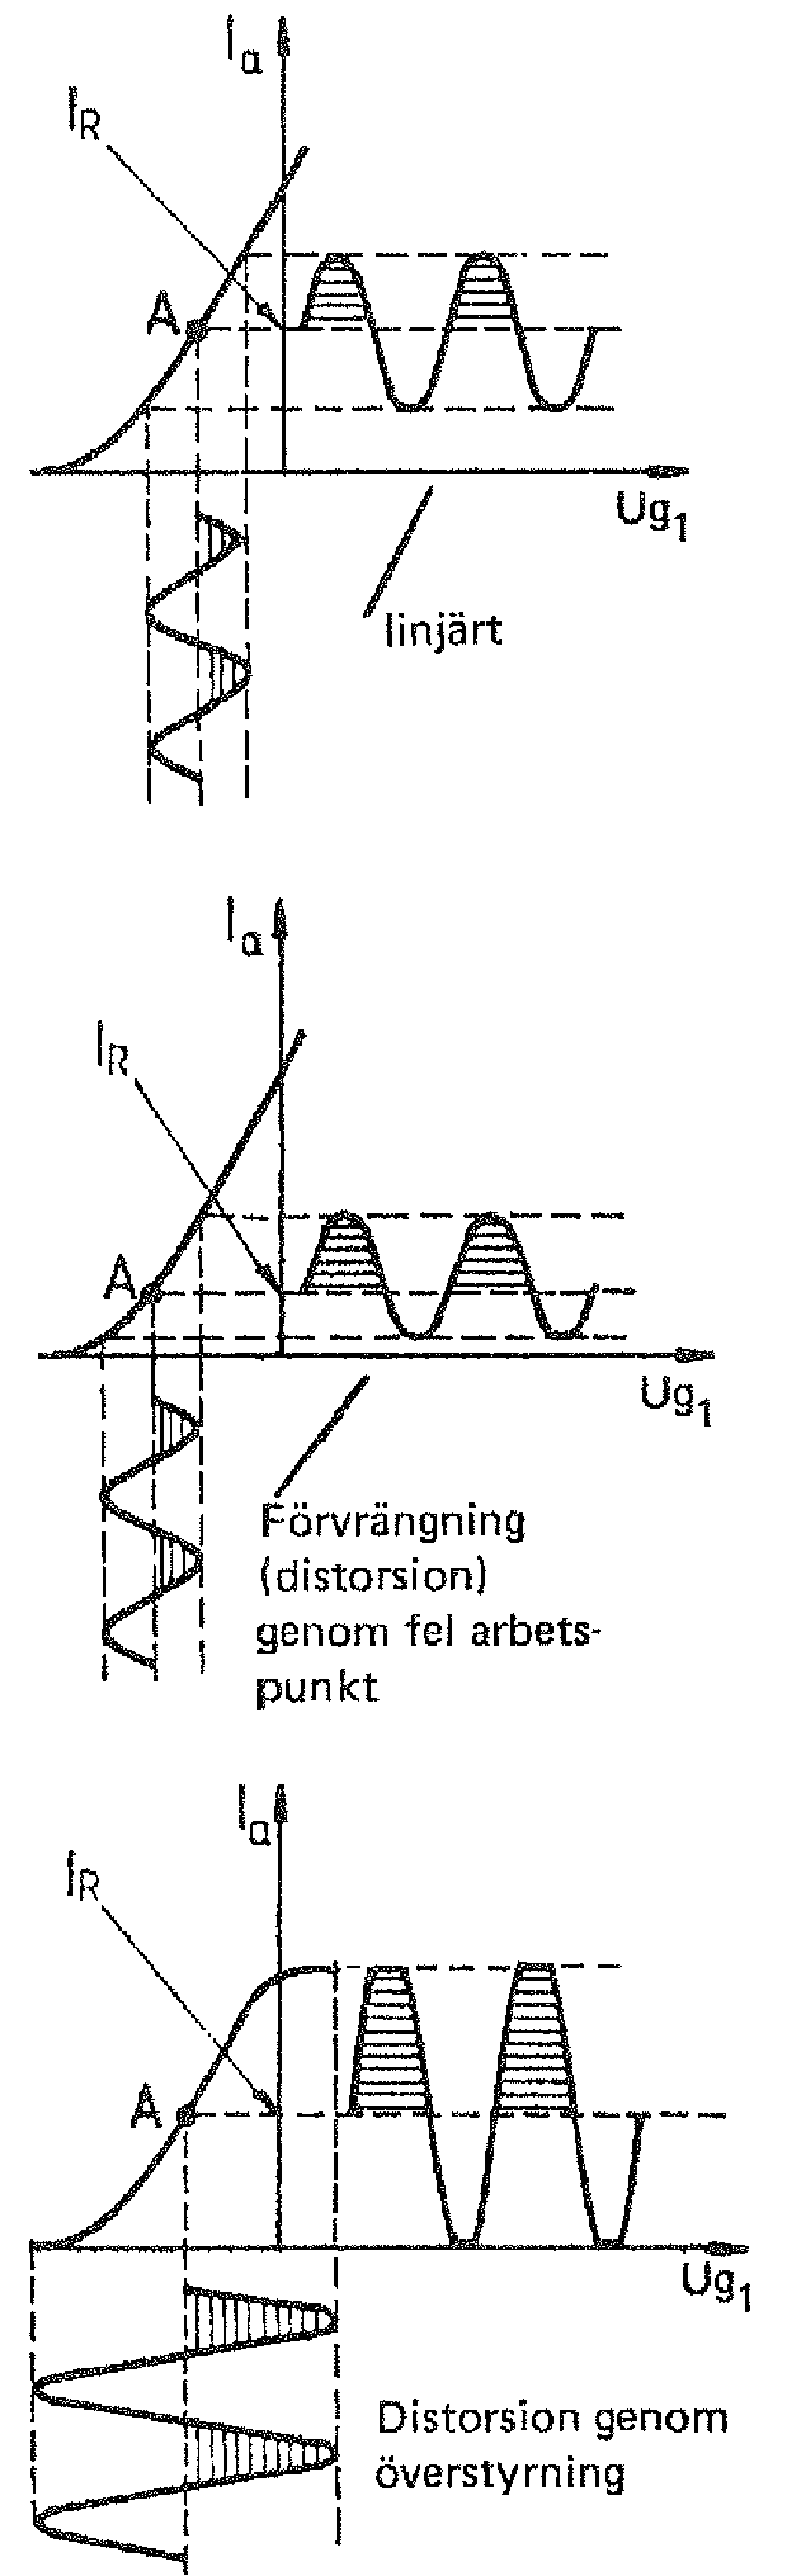
\includegraphics[width=0.3\textwidth]{images/cropped_pdfs/bild_2_3-44.pdf}
\caption{Förstärkare i klass A}
\label{fig:BildII3-44}
\end{wrapfigure}

\subsubsection{Klass A}
\index{klass A}

Bild \ref{fig:BildII3-44} illustrerar klass A är ett arbetssätt i linjära
LF- och HF-förstärkarsteg, till exempel i mottagare samt AM- och SSB-modulerade
sändare.
Vilovärdet på strömmen i huvudkretsen, den så kallade arbetspunkten, placeras i
mitten på den rakaste delen av styrkaraktäristikan (\(I=0,5\cdot I_{max}\)).
Därmed fås låg distorsion.
Verkningsgraden är upp till 50~\%.

\subsubsection{Klass AB}
\index{klass AB}

Klass AB är ett godtagbart linjärt arbetssätt för AM- resp. SSB-modulering,
men med en lägre viloström.
Arbetspunkten ligger mellan den för klass A och B.
Ett linjärt arbetssätt enligt klass A är visserligen önskvärt vid SSB, men
verkningsgraden är lägre.
Klass AB är en kompromiss med bättre verkningsgrad utan en alltför stor
distorsion.

\subsubsection{Klass B}
\index{klass B}

\begin{wrapfigure}{R}{0.5\textwidth}
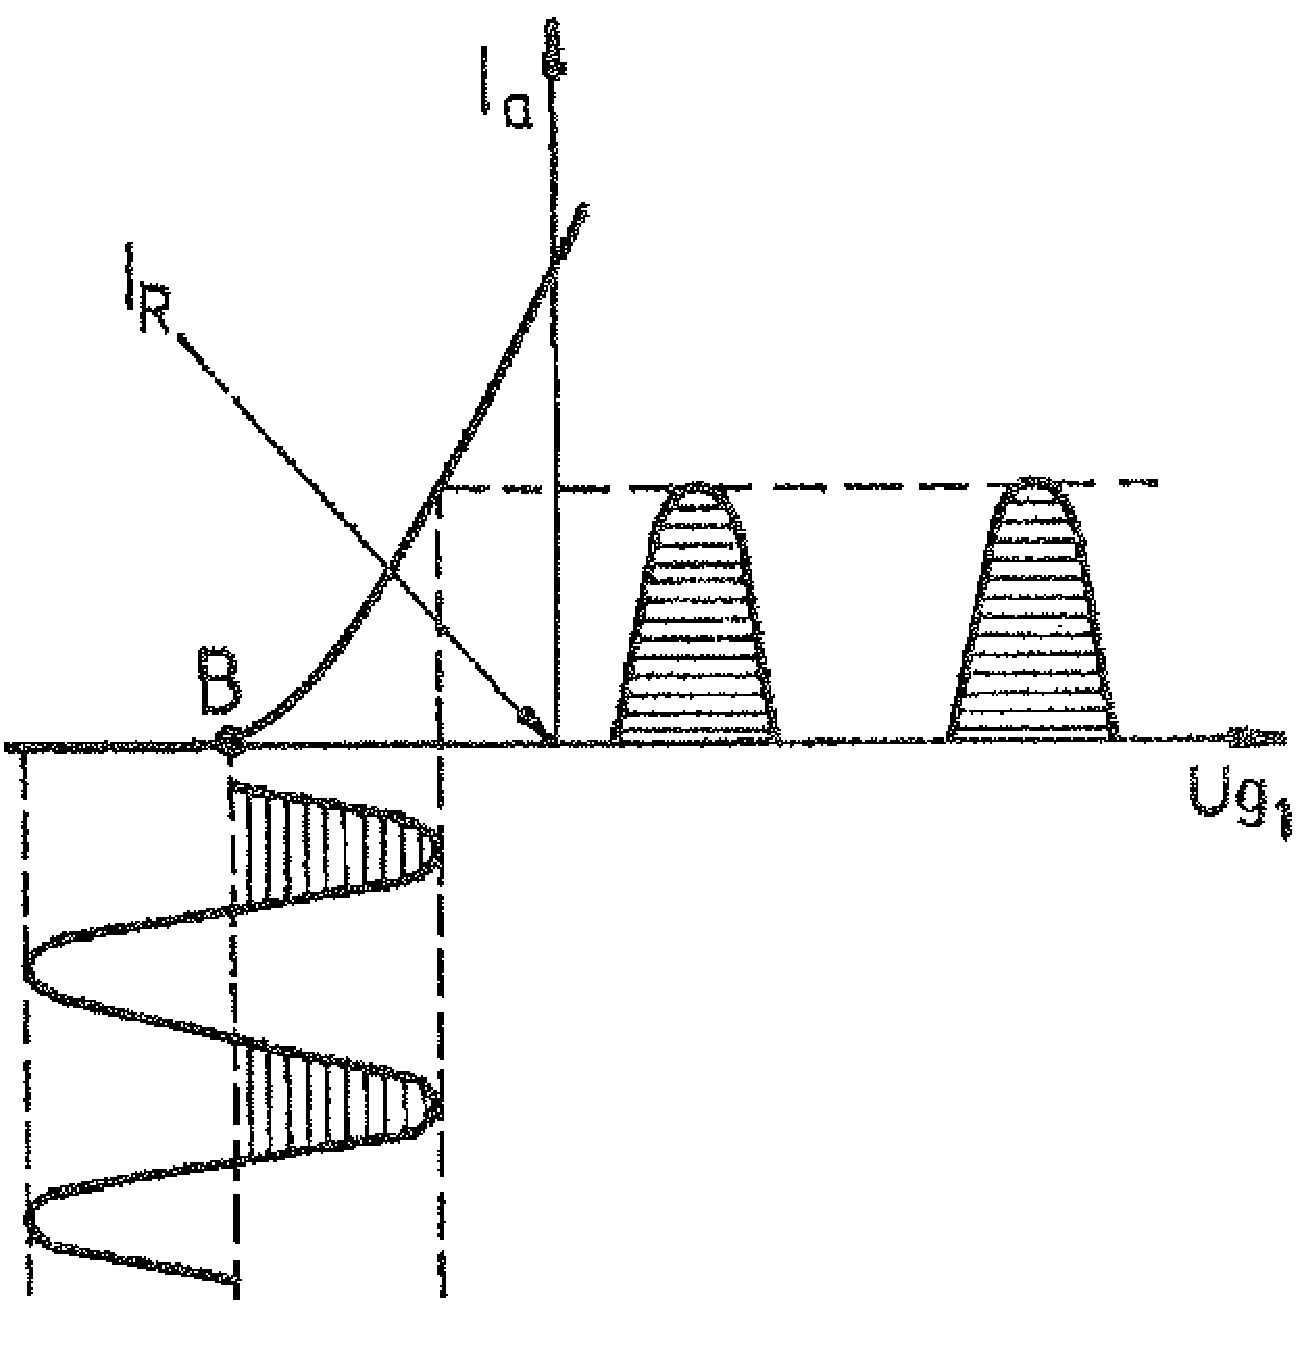
\includegraphics[width=0.5\textwidth]{images/cropped_pdfs/bild_2_3-45.pdf}
\caption{Förstärkare i klass B}
\label{fig:BildII3-45}
\end{wrapfigure}

Bild \ref{fig:BildII3-45}

Klass B är ett olinjärt arbetssätt med en låg viloström i förhållande
till \(I_{max}\) det vill säga arbetspunkten ligger i nederkant av
styrkaraktäristikans nedre krökta del. Verkningsgraden är upp till
67~\%. Trots det används klass B i linjära LF-och H F-förstärkarsteg
till exempel i SSB-sändare.

Om klass B skulle tillämpas i ett slutsteg med endast ett rör eller en
transistor skulle större delen av uteffekten förloras i splatter,
dvs. som förvrängda signaler långt vid sidan om den egentliga nyttosignalen.
Ett sätt att undvika det är att använda en avstämd utgångskrets med högt
Q-värde.
Linjär förstärkning kan också erhållas med två mottaktkopplade rör eller
transistorer i klass B.
Utgångskretsen behöver då inte vara avstämd av linjäritetsskäl.

\subsubsection{Klass C}
\index{klass C}

\begin{wrapfigure}{R}{0.5\textwidth}
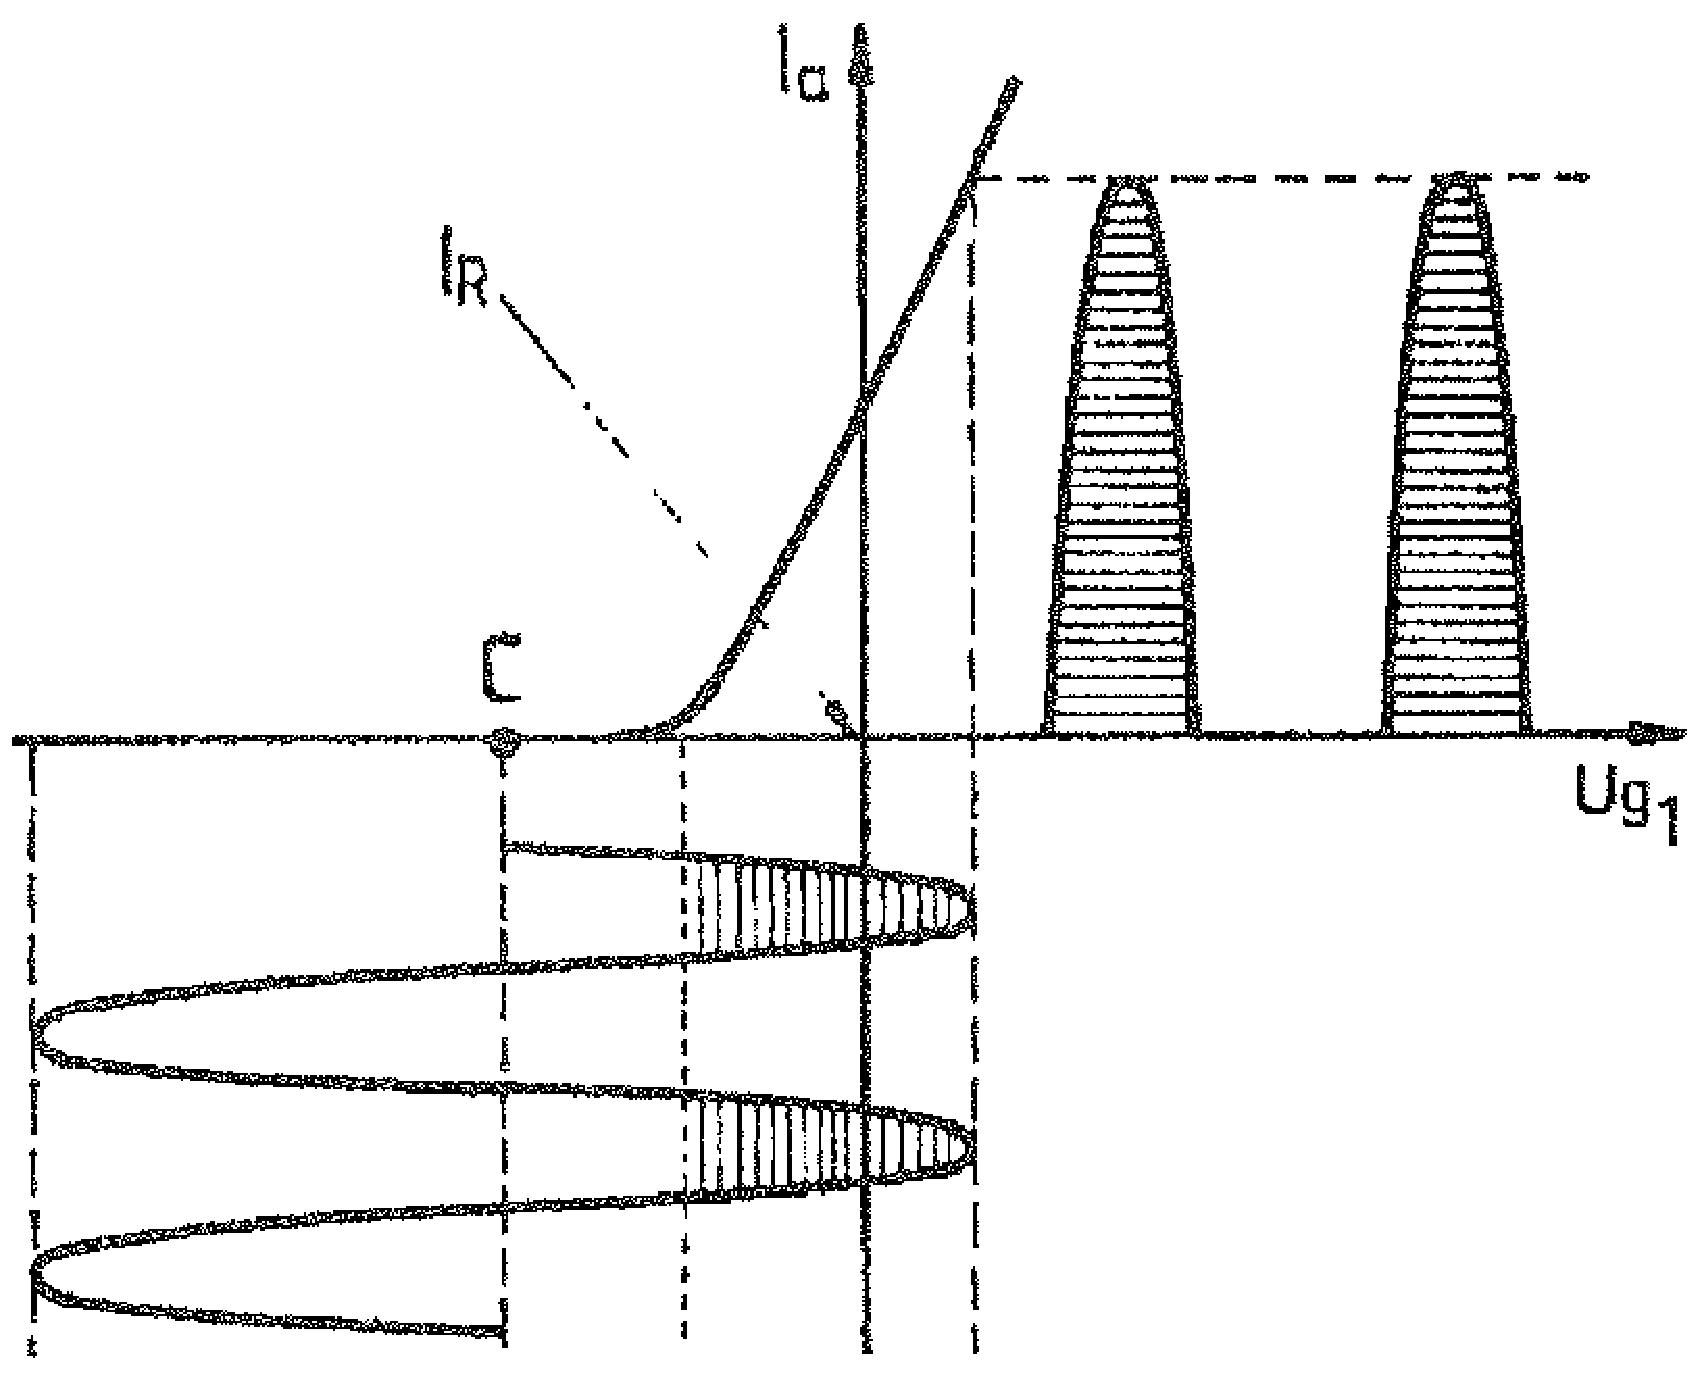
\includegraphics[width=0.5\textwidth]{images/cropped_pdfs/bild_2_3-46.pdf}
\caption{Förstärkare i klass C}
\label{fig:BildII3-46}
\end{wrapfigure}

Bild \ref{fig:BildII3-46} visar klass C som används i HF-förstärkarsteg i
FM-, CW- och AM-sändare.
Arbetssättet är kraftigt olinjärt.
Viloströmmen är noll, dvs. arbetspunkten ligger på den negativa delen av
styrkaraktäristikan.
Endast toppen av den ena halvvågen av insignalen återges och i starkt
förvrängd form.
Verkningsgraden är upp till 80~\%.
Övertonerna dämpas av svängningskretsen.
En resonanskrets med högt Q-värde behövs som utgångskrets varvid
amplituddistorsion inte framstår som besvärande vid CW och FM.
Med hjälp av en utgångskrets kan frekvensmultiplicering utföras med
förstärkare i klass C.
(På följande tre bilder är \(I_R\)=anodviloström.)

\subsection{Frekvensmultiplicering}
\index{frekvensmultiplicering}
\index{frequency multiplication}

\begin{figure}
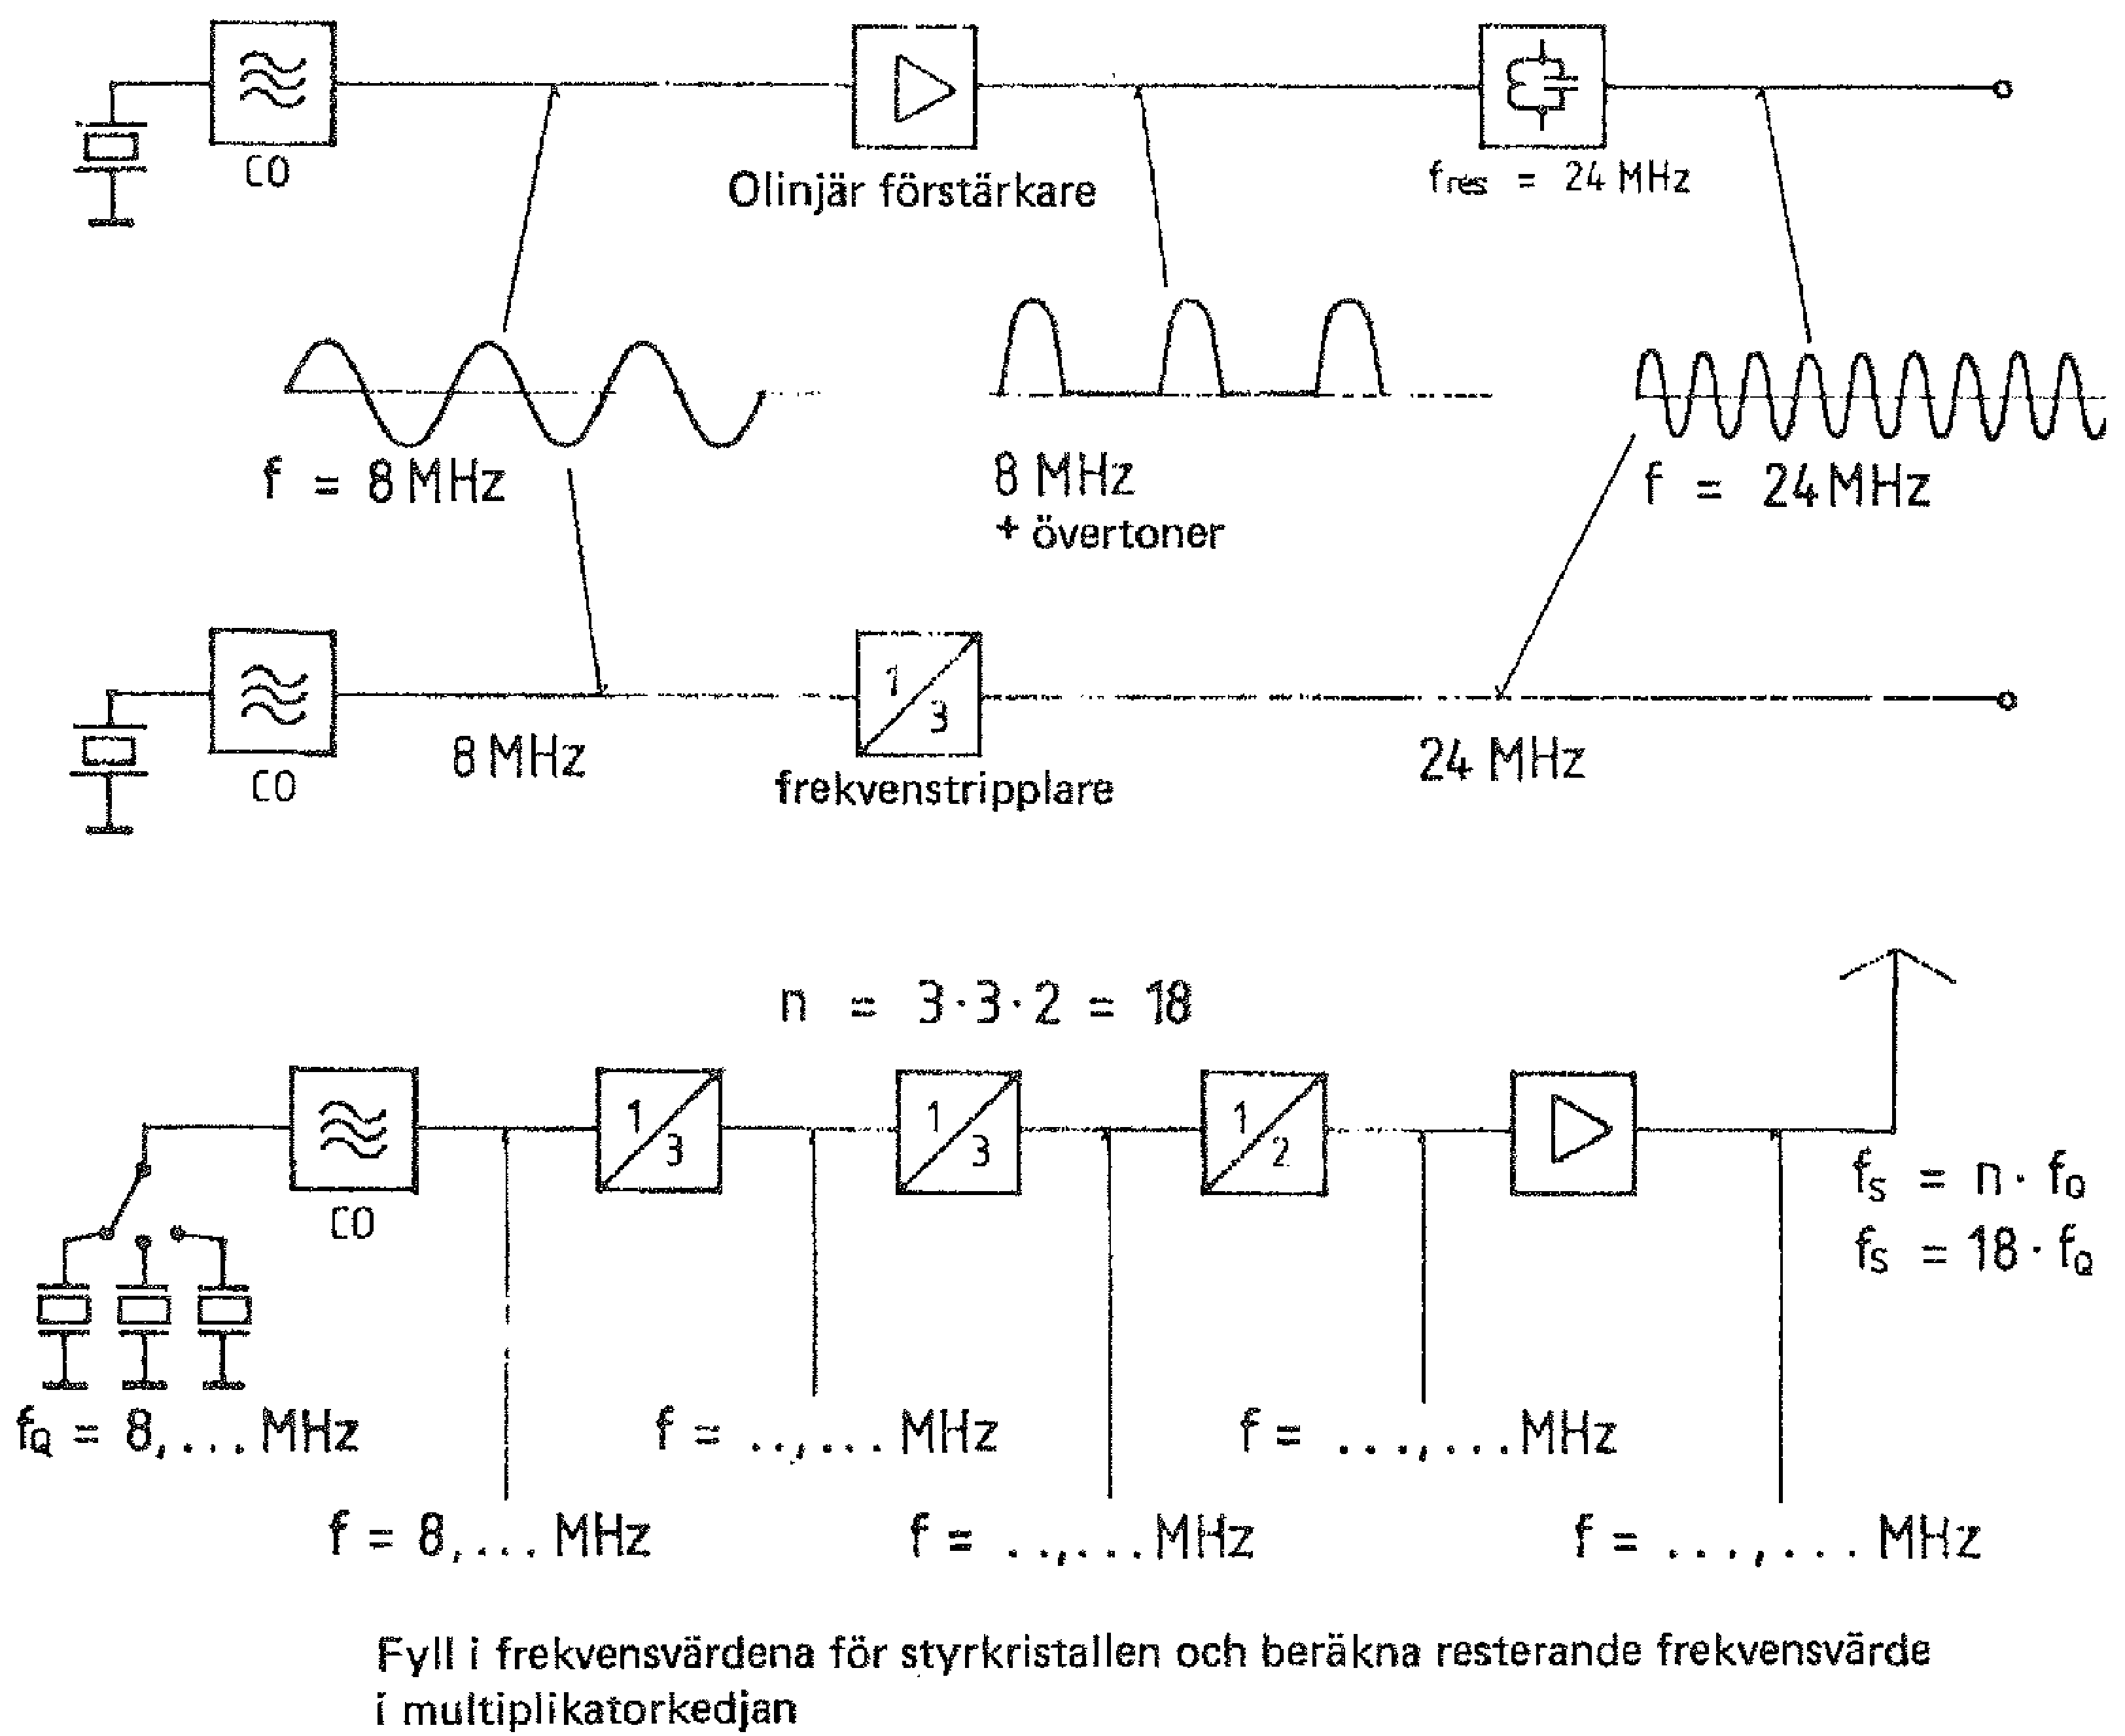
\includegraphics[width=\textwidth]{images/cropped_pdfs/bild_2_3-47.pdf}
\caption{Frekvensmultipliceringskedja}
\label{fig:BildII3-47}
\end{figure}

\emph{Frekvensmultiplicering} (eng. \emph{frequency multiplication}) kan
användas för att skapa en högre frekvens än den som avges av oscillatorn.
Bild \ref{fig:BildII3-47} visar hur oscillatorn följs då av ett eller flera
frekvensmultiplicerande förstärkarsteg som arbetar i klass C.

I utgången av ett frekvensmultiplicerande steg måste finnas en
svängningskrets, som är avstämd till önskad frekvens, dvs. överton
av insignalen.
Denna överton förstärks i efterföljande förstärkarsteg, vilket också kan vara
frekvensmultiplicerande.

Ju högre multiplikationsfaktorn är, desto högre förspänning krävs för
att svängningskretsen i utgången ska svänga obehindrat.
Med hög multipliceringsfaktor i ett enda steg dämpas signalen då så mycket att
en hög förstärkning behövs i efterföljande steg.
I praktiken anordnas därför en kedja av frekvensdubblande och
frekvenstripplande.
Den totala multipliceringsfaktorn är faktorerna för vartdera steget
multiplicerat med varandra.

Som exempel visar bilden blockschemat för en VHF-sändare med
oscillatorkristaller i 8~MHz-området.
Som räkneövning kan andra kristallfrekvenser sättas in för beräkning av den
slutlig sändningsfrekvensen.
I frekvensmultiplicerande sändare kan även slutsteget arbeta i klass C, vilket
är vanligt i sändare för telegrafi eller FM-telefoni.
För att då förhindra utsändning av alla de övertoner som alstras i
förstärkarkedjan, så förses slutstegets utgång med en svängningskrets som är
avstämd till sändningsfrekvensen.
Övertonsdämpningen kan förbättras ytterligare med ett efterföljande
lågpassfilter.
Övertoner för 144~MHz är 288~MHz, 432~MHz osv.

Frekvensmultiplicering behöver nödvändigtvis inte göras med ett förstärkarsteg
i klass C.
En diod har nämligen olinjär karaktäristik och därmed alstras det övertoner i
de strömmar som passerar genom den.
En av dessa övertoner kan filtreras fram och förstärkas.
Till exempel finns det frekvenstripplingssteg byggda kring en speciell typ av
kapacitansdiod -- varaktordiod.
Vanliga frekvensområden för så kallad varaktortripplare är 144/432~MHz och
432/1296~MHz.

Såväl signalen från en kristalloscillator som den från en VFO kan
multipliceras till en högre frekvens.

Förr täckte VFO i amatörradiosändarna oftast frekvensområdet 3,5--3,8~MHz.
Med en så vald VFO-frekvens kunde alla upplåtna frekvensband för
amatörradio nås med frekvensmultiplicering.
De ursprungliga amatörradiobanden i KV-området ligger fortfarande harmoniskt
relaterade av detta skäl.

Således
\begin{align*}
  3,5 \cdot 2 & = 7\ \text{MHz} \\
  3,5 \cdot 2 \cdot 2 & = 14\ \text{MHz} \\
  3,5 \cdot 2 \cdot 3 & = 21\ \text{MHz} \\
  3,5 \cdot 2 \cdot 2 \cdot 2 & = 28\ \text{MHz} \\
\end{align*}

Vid frekvensmultiplicering flerfaldigas inte bara oscillatorfrekvensen utan
även variationerna i den.
Om till exempel VFO-frekvensen i området 3,5~MHz ändras med 50~Hz, så ändras
utfrekvensen i området 28~MHz med \(2 \cdot 2 \cdot 2 \cdot 50 = 400\) Hz.
Alla frekvenser i signalen multipliceras på detta sätt.
Amplitudmodulerad telefoni kan därför inte överföras genom en
frekvensmultipliceringskedja utan att talet förvrängs.

\subsection{Sändarslutsteg}
\textbf{HAREC a.\ref{HAREC.a.2.8.2}\label{myHAREC.a.2.8.2}}
\index{slutsteg}
\index{förstärkare!slutsteg}

\subsubsection{Slutsteg med en transistor}

\begin{wrapfigure}{R}{0.5\textwidth}
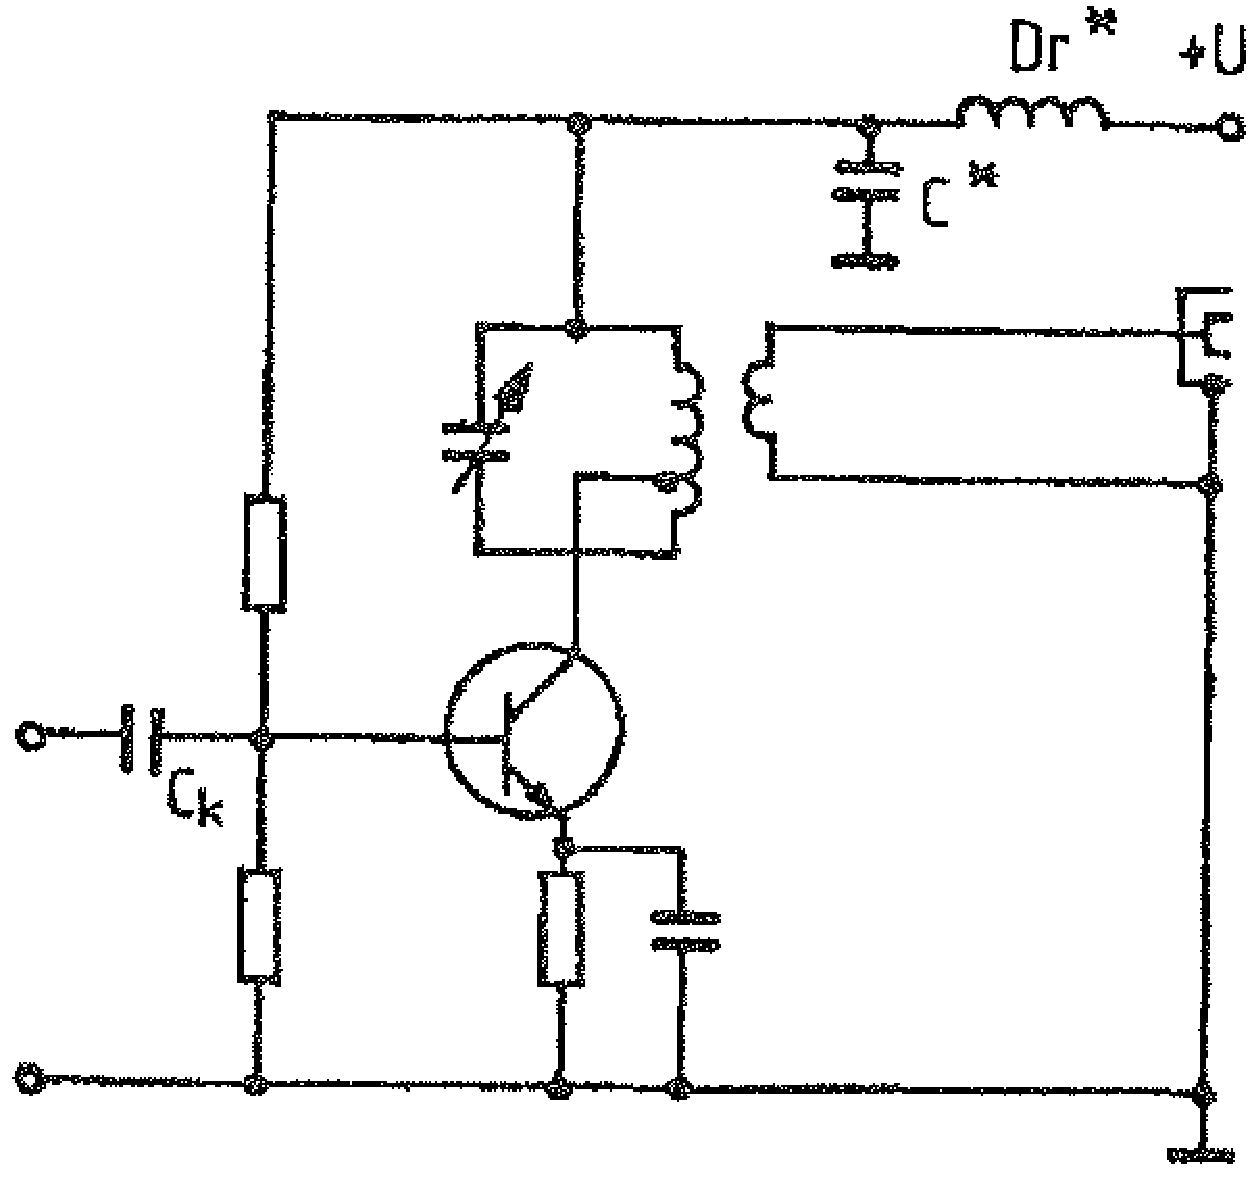
\includegraphics[width=0.5\textwidth]{images/cropped_pdfs/bild_2_3-48.pdf}
\caption{Slutsteg med en transistor}
\label{fig:BildII3-48}
\end{wrapfigure}

Transistorslutsteg för HF byggs vanligen emitterkopplade på grund av den
högre effektförstärkningen.
Moderna LDMOS-transistorer kan lämna en kilowatt.

Bild \ref{fig:BildII3-48} visar ett sådant förstärkarsteg.
Kollektorbelastningen består av en svängningskrets.
För att anpassa transistorns kollektorimpedans till svängningskretsens
impedans, har kollektorn anslutits till ett uttag på svängningskretsens spole.

Drossel \(Dr\) och kondensator \(C\) fungerar som en HF-mässig
avkoppling av strömförsörjningen.
Uteffekten tas ut från svängningskretsen över en kopplingslindning med samma
impedans som belastningen.
För linjär återgivning krävs drift i klass A eller möjligen klass AB.

\subsubsection{Slutsteg med två transistorer}
\index{mottaktskopplat slutsteg}
\index{slutsteg!mottaktskopplat}
\index{push-pull amplifier}

\begin{figure}
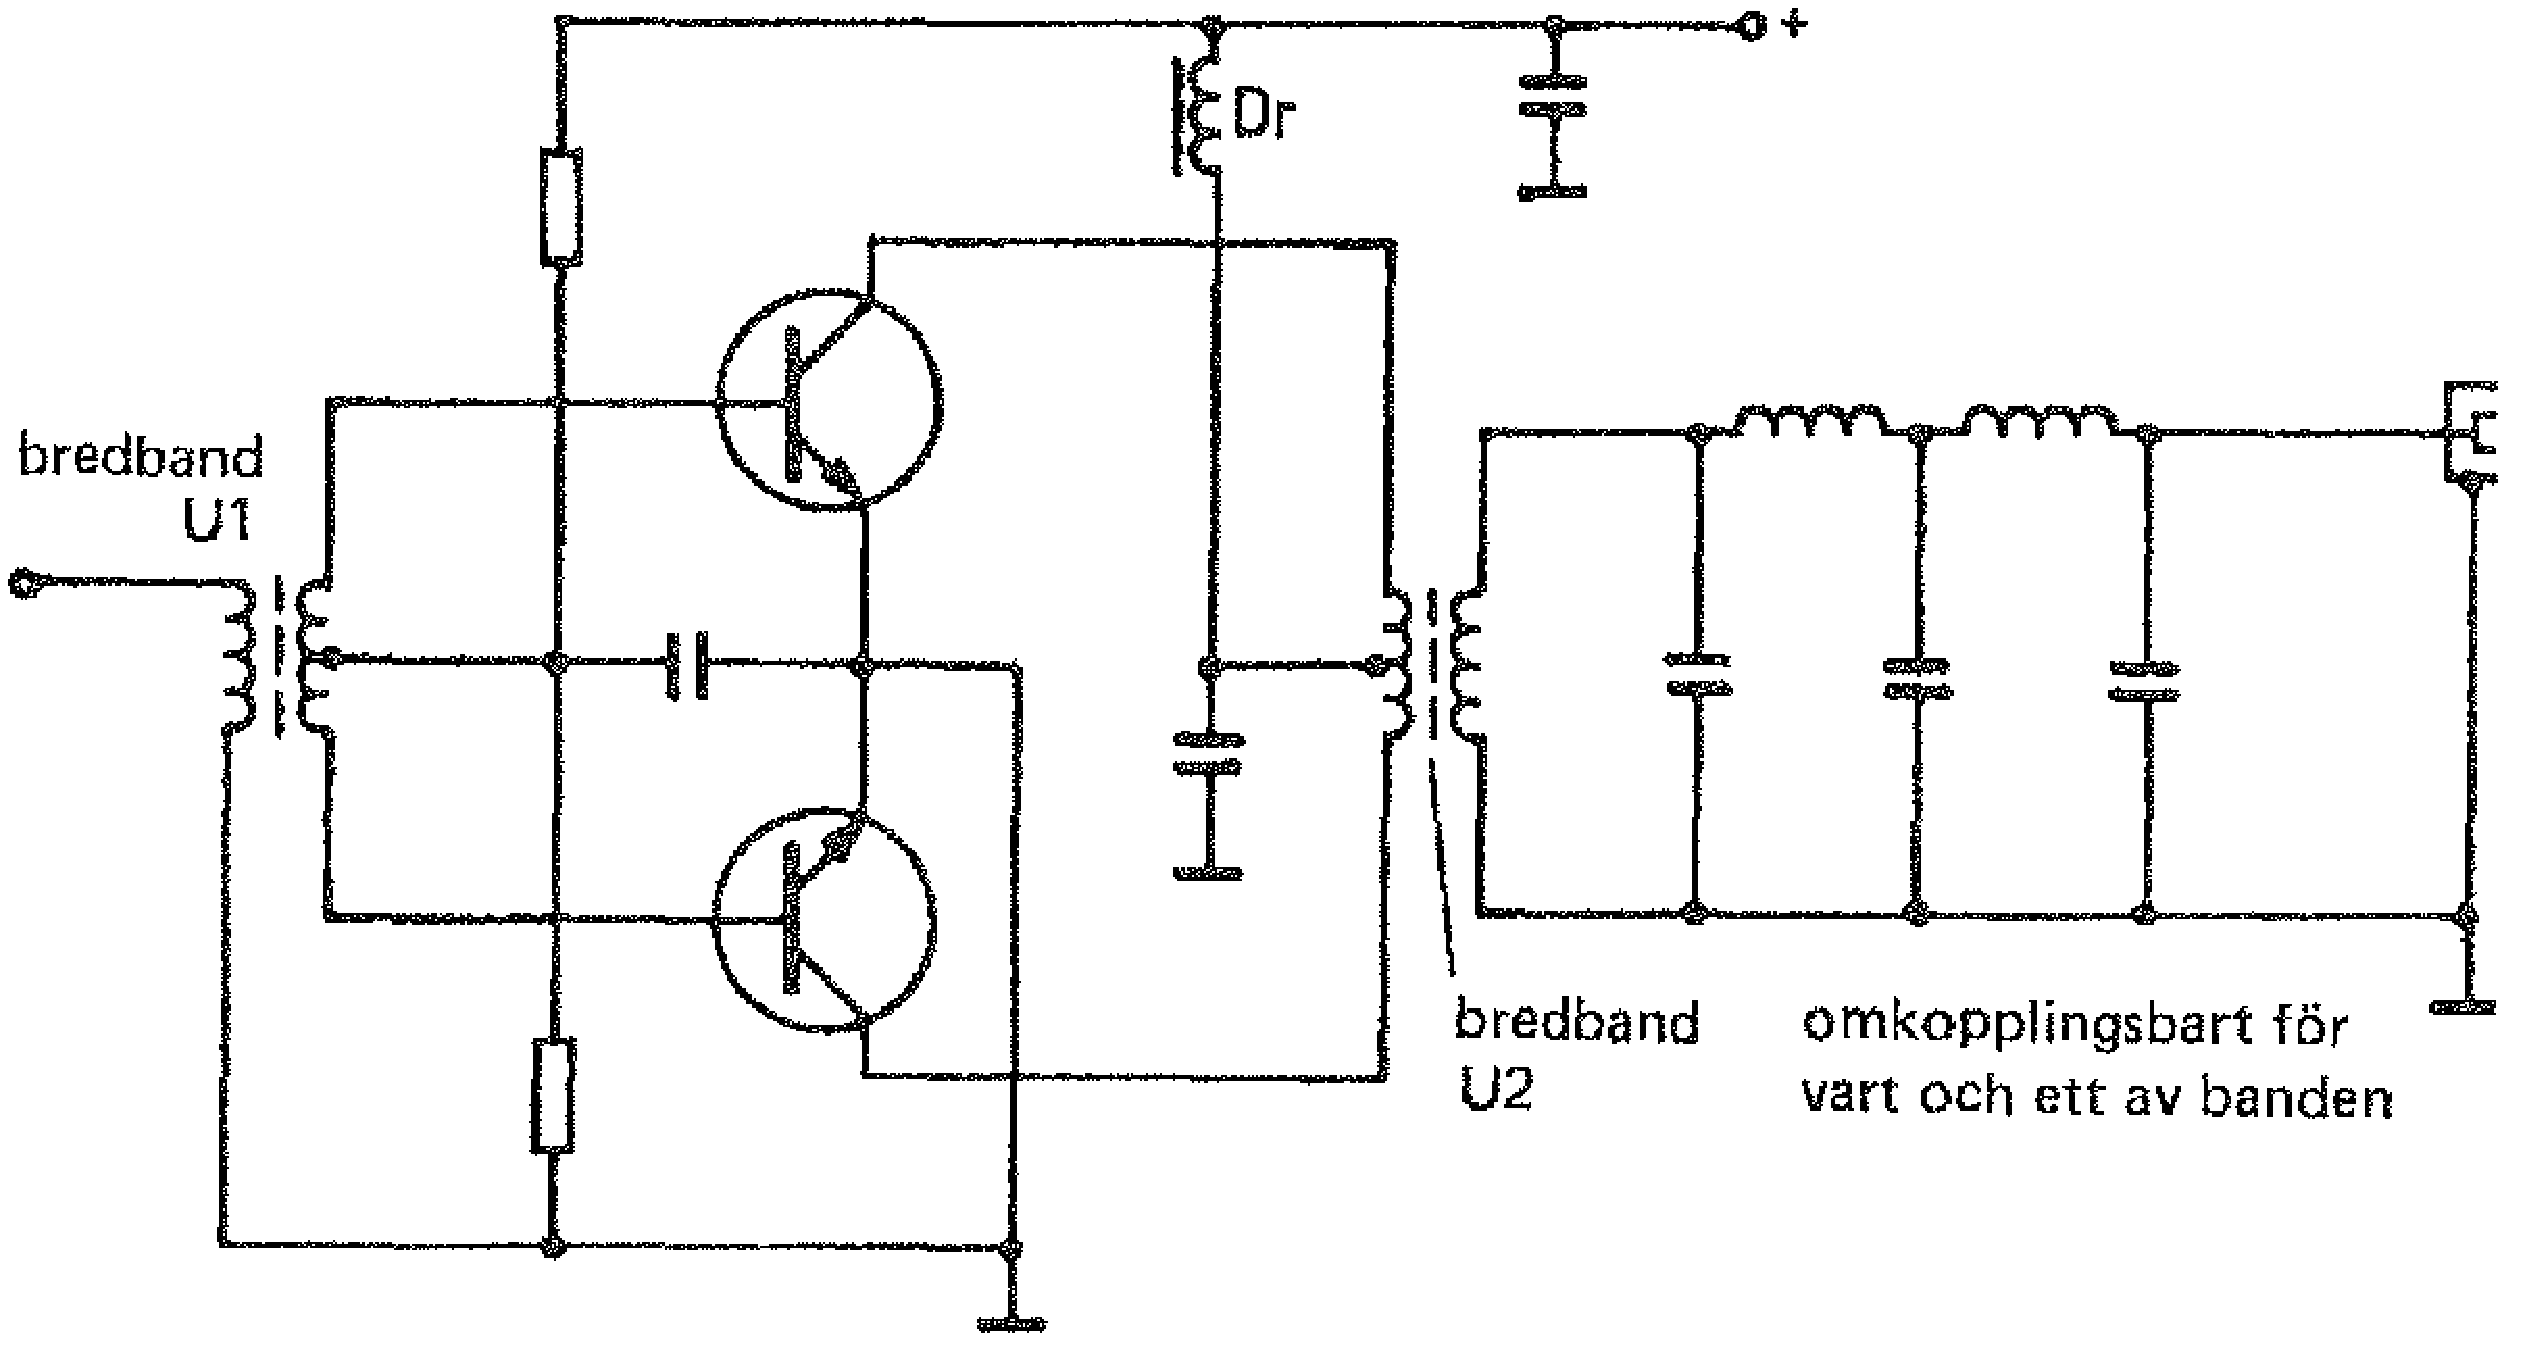
\includegraphics[width=\textwidth]{images/cropped_pdfs/bild_2_3-49.pdf}
\caption{Mottaktskopplat slutsteg med transistorer}
\label{fig:BildII3-49}
\end{figure}

Bild \ref{fig:BildII3-49} visar ett \emph{mottaktkopplat} (eng.
\emph{push-pull amplifier}) förstärkarsteg i klass B har god verkningsgrad
samtidigt som det är nöjaktigt linjärt för SSB i amatörradio.
I ett slutsteg med endast en transistor skulle denna behöva klara fyra gånger
så stor förlusteffekt.

På grund av de låga impedansvärdena i transistoriserade förstärkarsteg används
transformatorer, vilka inte är frekvensselektiva och därför inte dämpar
övertoner.
Med mottaktkopplingen alstras dock inte jämna övertoner.
För övertonsdämpning används fast avstämda bandpassfilter, ofta ett per
frekvensband, mellan drivsteg och slutsteg samt mellan slutsteg och antenn.

För noggrann anpassning till antennen behövs en antennkopplare --
så kallad matchbox -- med ett \(\pi \)-, T- eller L-kopplat LC-filter.

Att ett slutsteg är ''bredbandsavstämt'' är således en fråga om definitioner.

\subsubsection{Högeffektslutsteg med en tetrod}

\begin{figure}
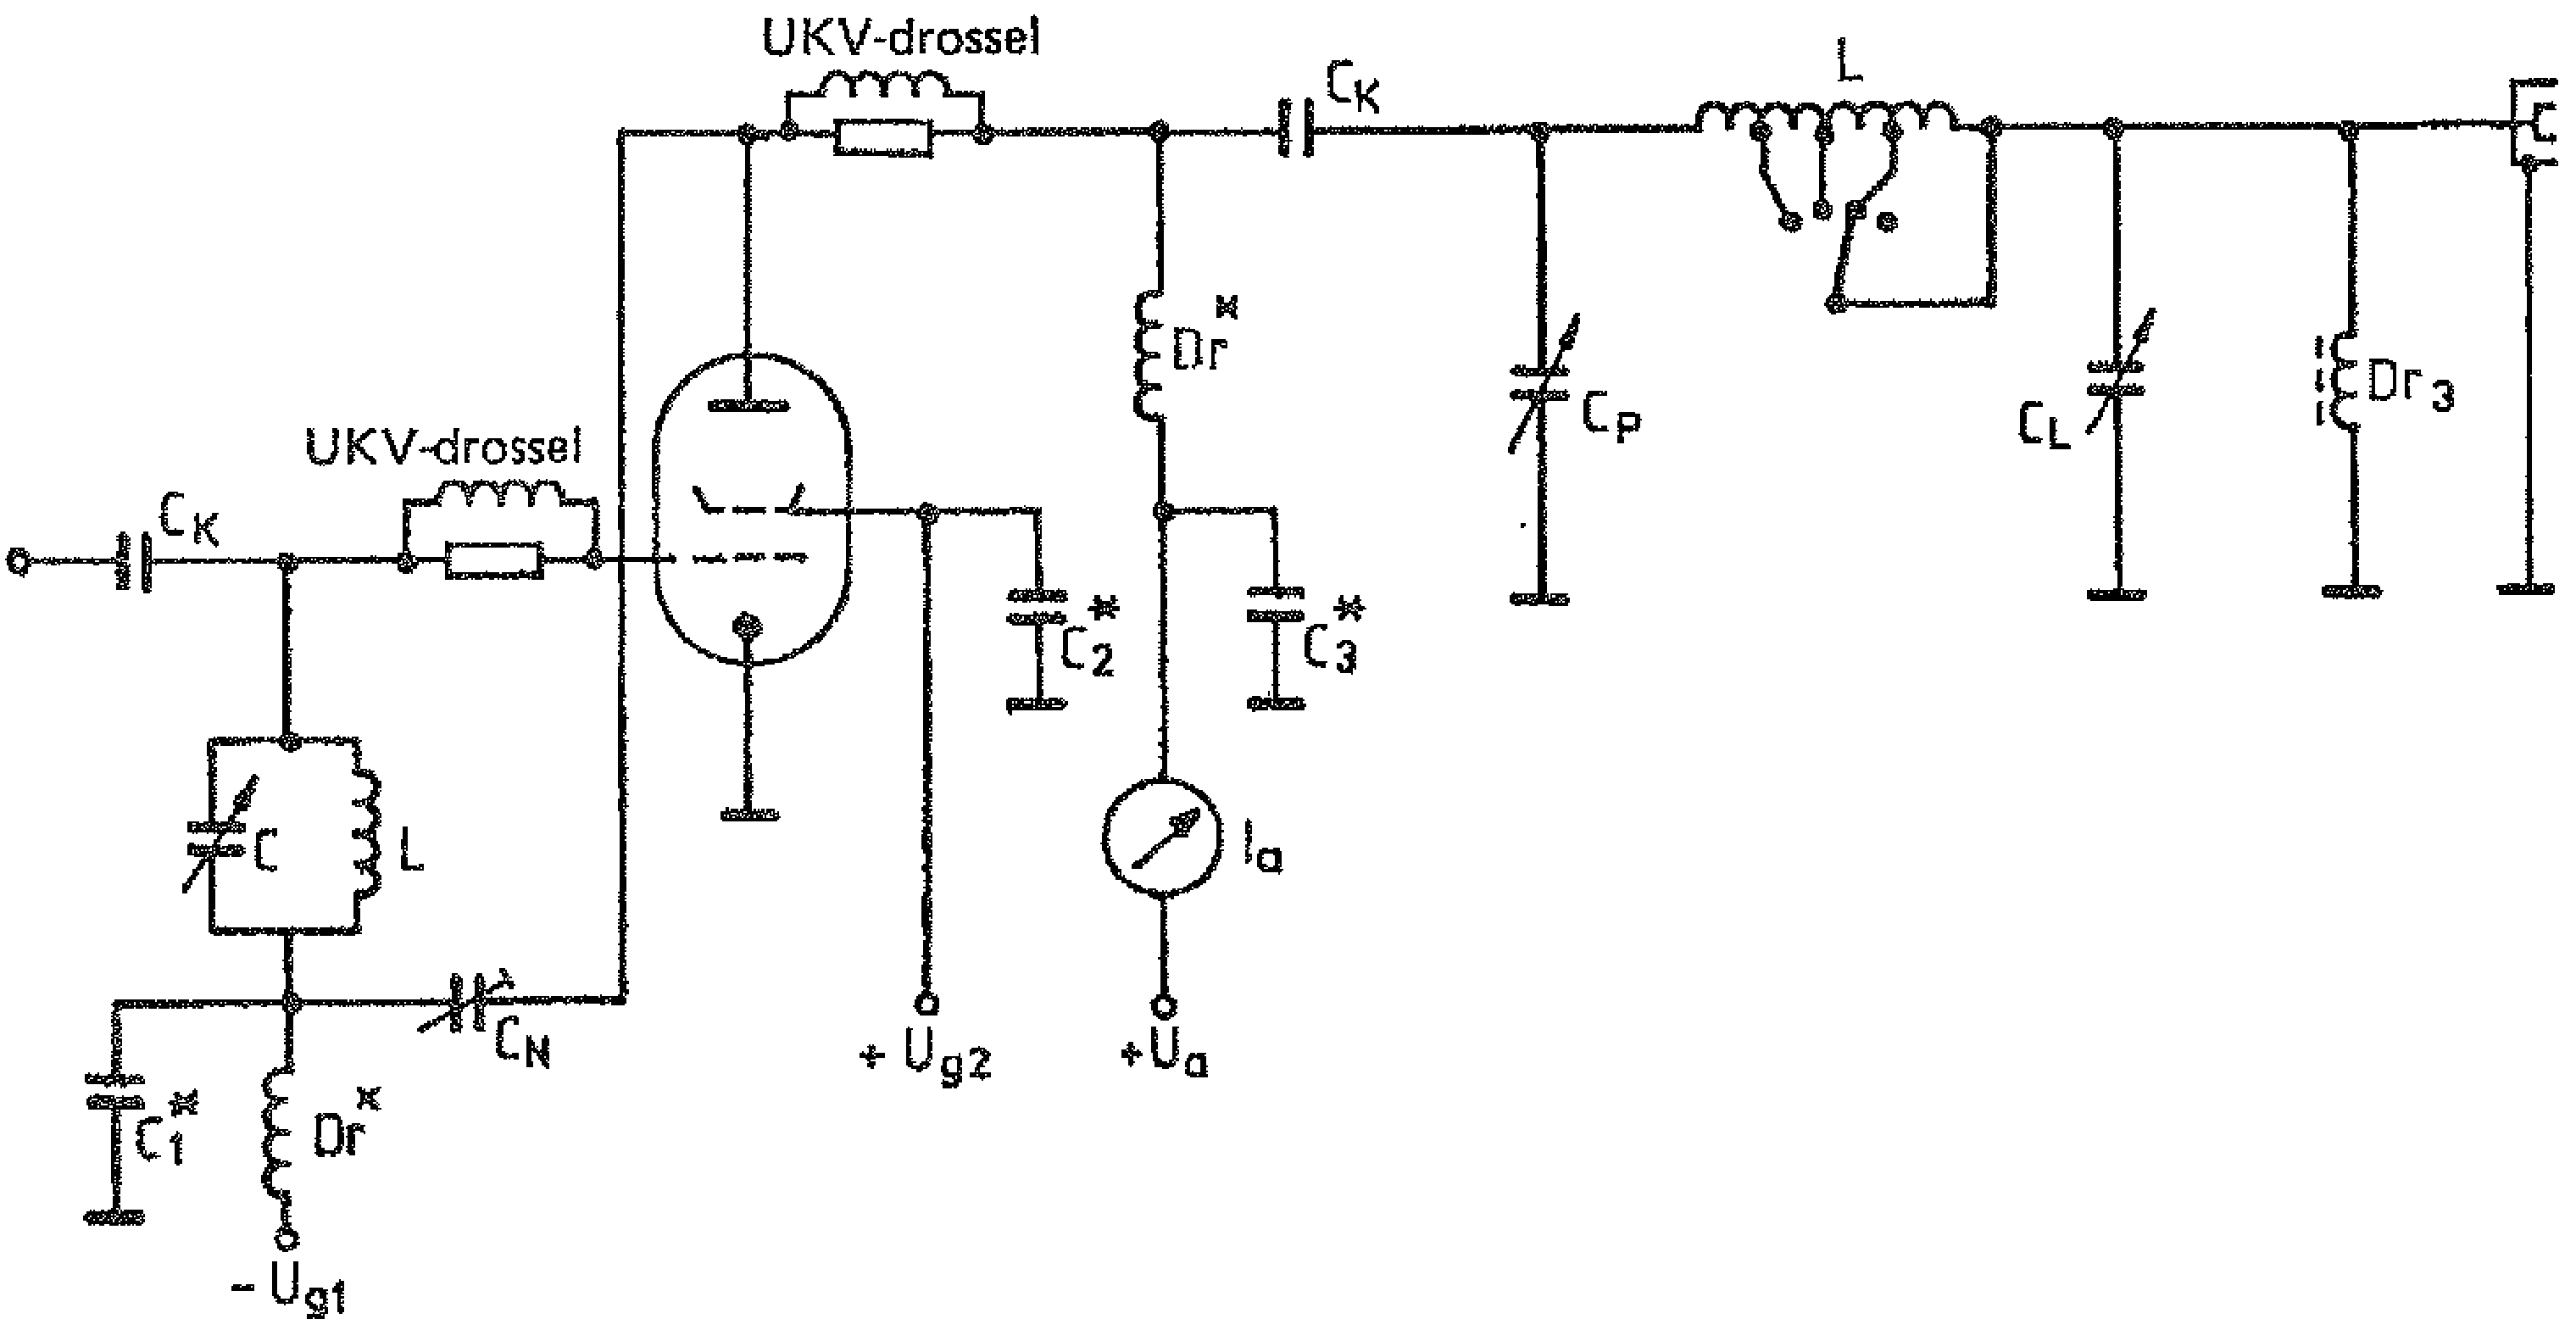
\includegraphics[width=\textwidth]{images/cropped_pdfs/bild_2_3-50.pdf}
\caption{Högeffektslutsteg med en tetrod}
\label{fig:BildII3-50}
\end{figure}

Bild \ref{fig:BildII3-50} visar ett effektslutsteg för HF med ett elektronrör,
en så kallad tetrod, i katodkoppling.
Det kan även vara en triod eller en pentod.

Med LC-kretsen i styrgallerkretsen filtreras (selekteras) önskade
signalfrekvens ut ur signalerna från föregående steg.

Drosslarna \(Dr\) spärrar HF och kondensatorerna \(C_1\), \(C_2\) och
\(C_3\) kortsluter (avkopplar) HF till jord.
Allt för att hindra HF att komma in i kraftaggregatet.

HF-förstärkare kan råka i oönskad självsvängning.
Orsakerna kan vara många, bland annat dålig avkoppling av matningsspänningar,
induktiv och/eller kapacitiv återkoppling i kretsarna med mera.

Återkopplingsvägar både före och efter röret kan bilda oavsiktliga
svängningskretsar, som genererar självsvängning, ofta på mycket höga
frekvenser till exempel i VHF-området.
Sådana så kallade parasitsvängningar kan stoppas/dämpas med UHF-drosslar (UHF
Dr) omedelbart intill röranslutningarna.

En åtgärd mot självsvängning i elektronrör är en motkopplingsväg från anod till
styrgaller över en trimningsbar så kallad neutraliseringskondensator \(C_N\).
Slutstegets utgångskrets kan utformas på olika sätt.
Bilden visar ett numera vanligt sätt, det så kallade \(\pi\)-filtret (utläses
pi-), som fungerar som
\begin{itemize}
  \item en svängningskrets som är avstämd till sändningsfrekvensen
  \item ett övertonsdämpande lågpassfilter
  \item anpassning mellan rörets utgångsimpedans och antenntilledningens impedans.
\end{itemize}

\subsection{Högeffektslutsteg med två gallerjordade trioder (elektronrör)}

\begin{figure}
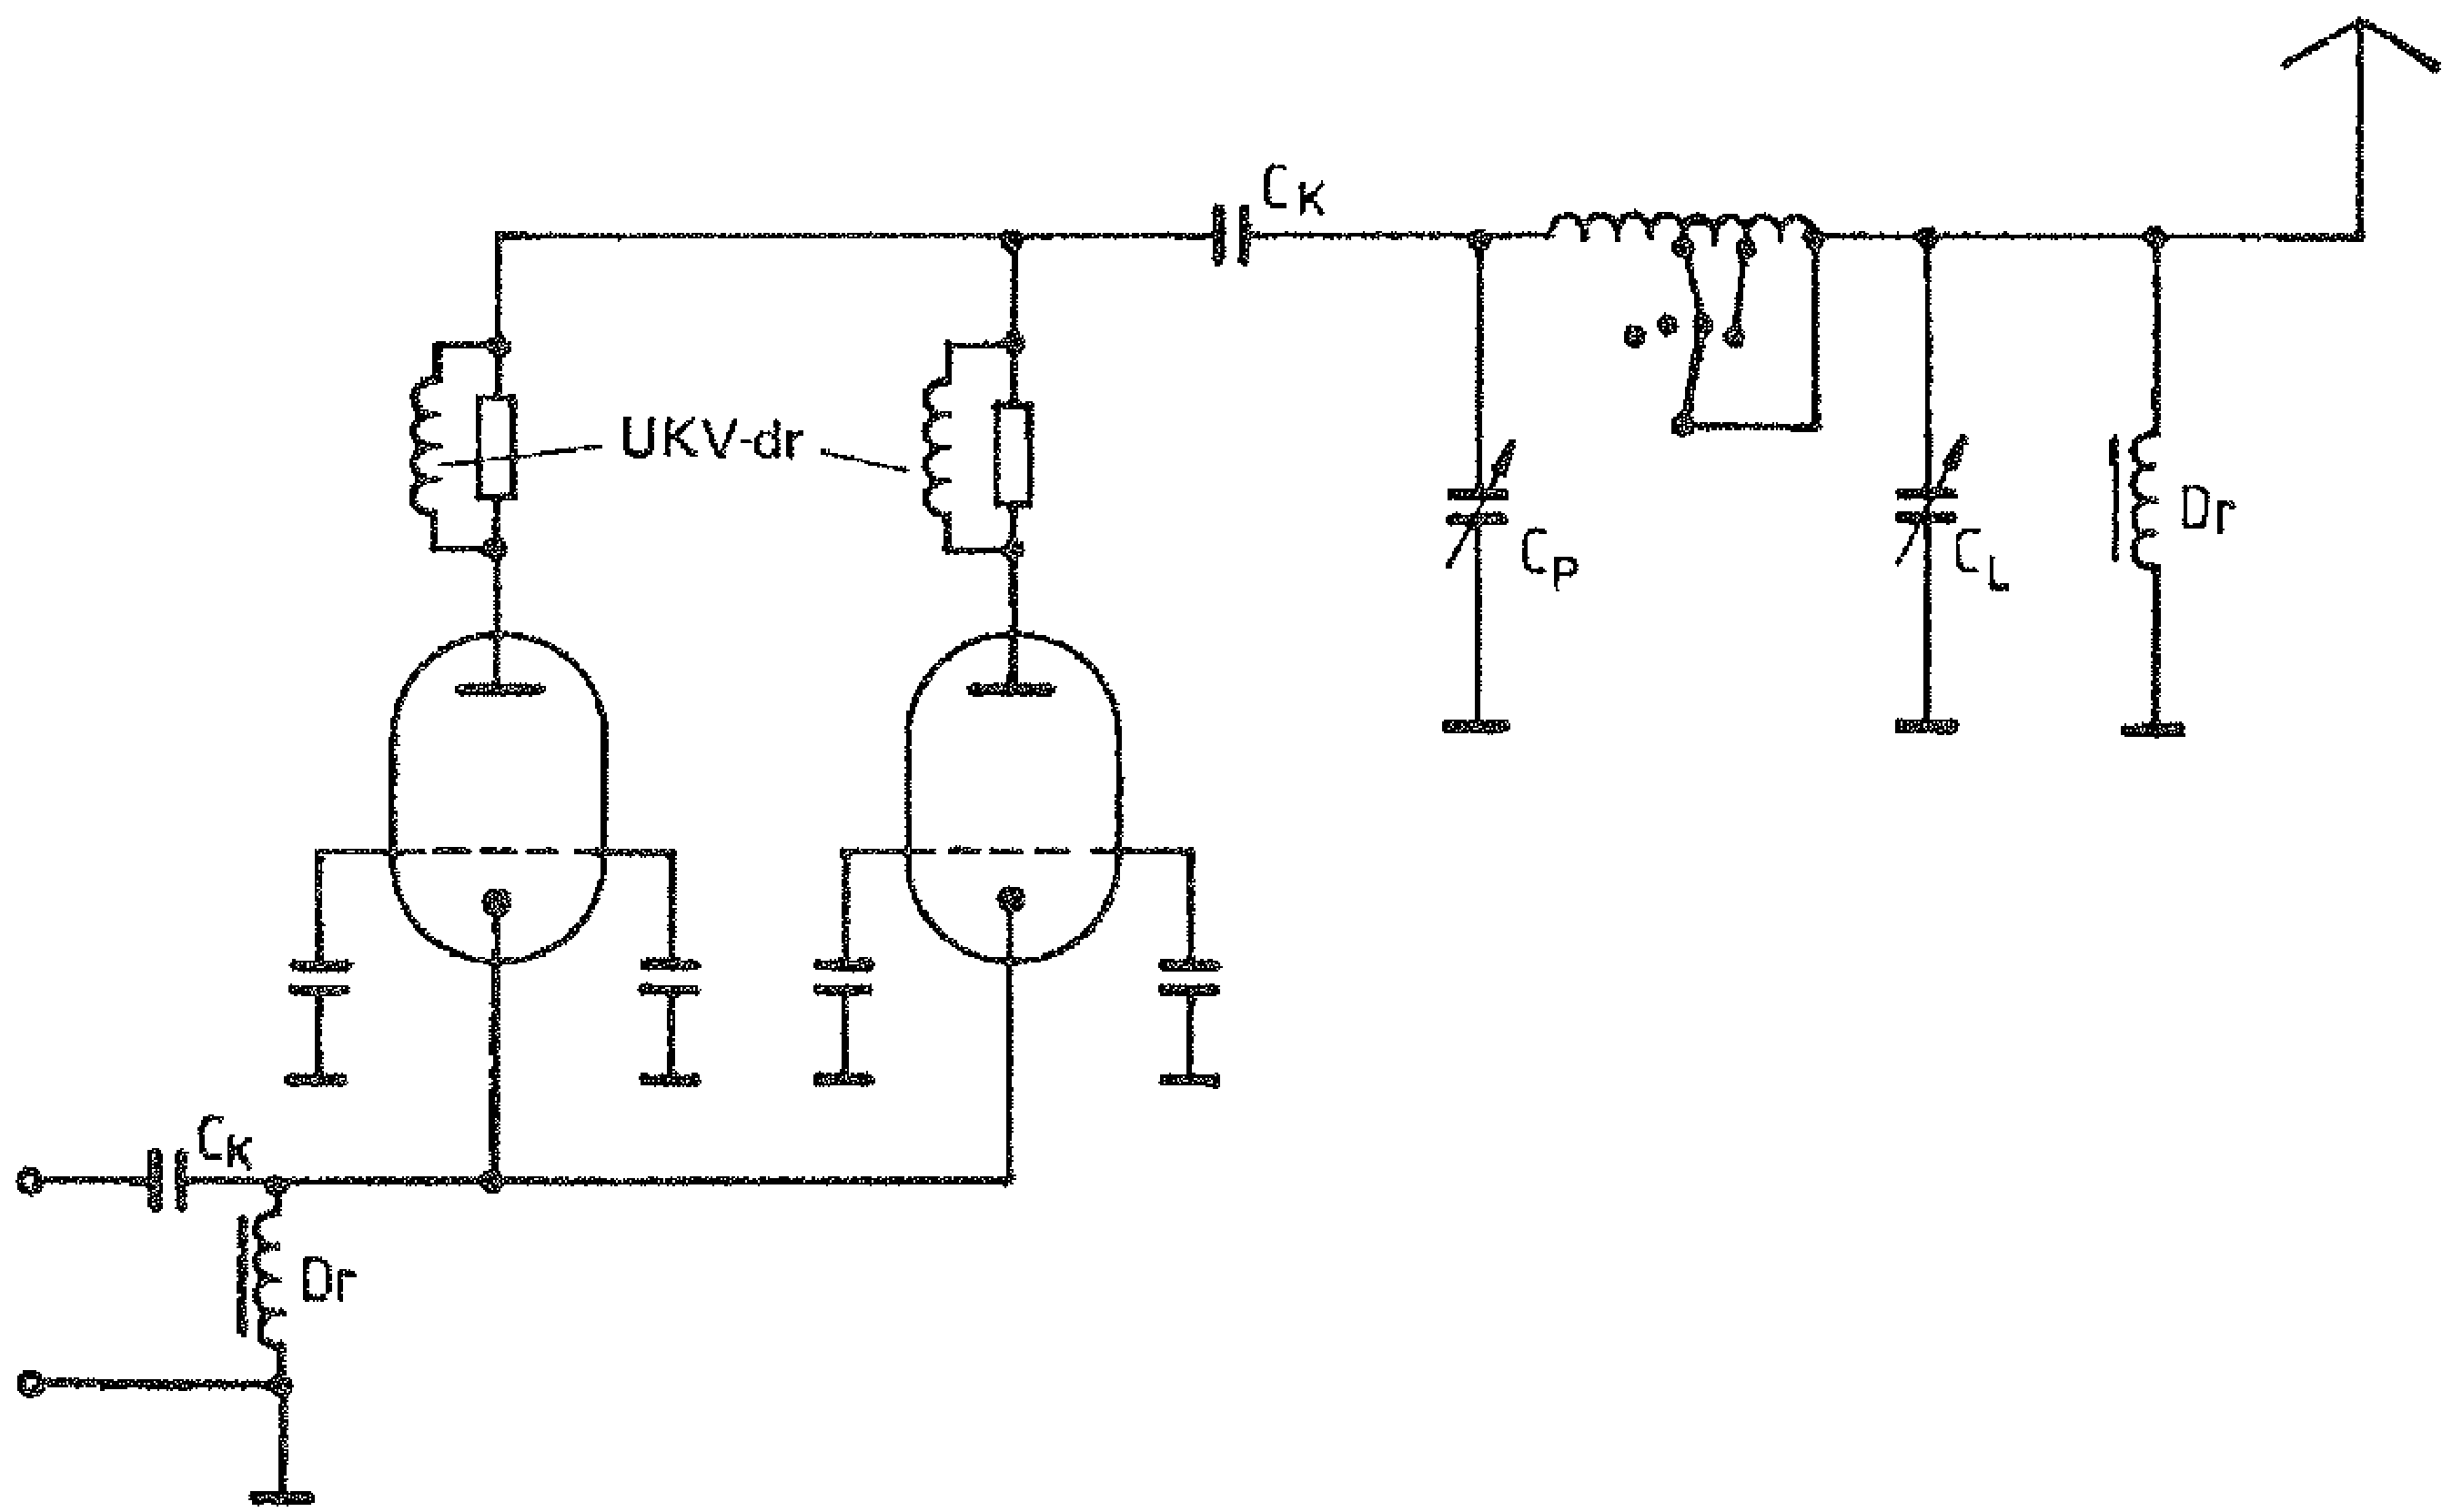
\includegraphics[width=\textwidth]{images/cropped_pdfs/bild_2_3-51.pdf}
\caption{Högeffektslutsteg med två trioder}
\label{fig:BildII3-51}
\end{figure}

Bild \ref{fig:BildII3-51} visar en gallerjordad koppling med två trioder.
Gallerjordad koppling innebär att elektronrörets styrgaller ligger på
HF-mässig nollpotential medan styrsignalen matas in på katoden.
Likspänningen mellan katod och styrgaller väljs så att rörets arbetspunkt blir
den avsedda.

Gallerjordad koppling passar särskilt för slutsteg med höga effekter,
men fordrar en högre styreffekt än andra kopplingar.
I gengäld ''överförs'' styreffekten till utgången via röret och ingår där i
uteffekten.
I gallerjordad koppling är kapacitansen låg mellan katod och anod, dvs.
mellan in- och utgång.
Därmed är risken för självsvängning betydligt mindre än i ett katodjordat steg.

Uteffekten kan ökas genom att parallellkoppla två eller flera rör, som då ska
ha så lika data som möjligt.
Uteffekten står i direkt proportion till antalet rör.

Flera parallellkopplade rör medför emellertid ökade totala rörkapacitanser,
ökade kapacitanser i kopplingsledningarna med mera, vilket är till nackdel vid
höga frekvenser.

Ett enda slutrör för hela effekten är emellertid dyrare än flera små
med tillsammans jämförbar effekt.
Mottaktkoppling av två rör (eng. ''push-pull'') i stället för parallellkoppling
har en fördel i högre förstärkning, men nackdelar i mer komplicerad
bandomkoppling av svängningskretsar med mera.
I moderna rörutrustade slutsteg för amatörradio förekommer därför endast ett
slutrör eller flera parallellkopplade.
Utgångskretsen är i regel ett \(\pi \)-filter med manuell eller automatisk
avstämning.

\subsection{Slutsteg med elektronrör jämfört med transistoriserade slutsteg}

Ett slutsteg med transistorer är kompakt och skaktåligt och använder
bara klenspänningar.
Det är därför särskilt väl lämpat för portabelt och mobilt bruk.

Men transistorer är känsliga för överbelastning.
Redan ytterst kortvarig överbelastning eller överspänning kan förstöra dem.
Transistorer är också känsliga för termisk överbelastning.
Särskilt vid höga effekter i trånga utrymmen är det nödvändigt med god kylning,
eventuellt med fläkt.

Ett slutsteg med elektronrör är inte så skaksäkert, men är mycket okänsligare
i övriga avseenden.
En nackdel är att det behövs extra effekt för uppvärmning av rörens katoder
samt höga anodspänningar, som är farliga vid ovarsamhet.
På grund av behovet av flera olika spänningar är även strömförsörjningen för
ett slutsteg med elektronrör mer komplicerad och omfångsrik.

\subsection{Toppvärdeseffekt PEP}
\textbf{HAREC a.\ref{HAREC.a.1.9.6}\label{myHAREC.a.1.9.6}}
\index{toppvärdeseffekt}
\index{effekt!toppvärdes}
\index{PEP}
\index{effekt!PEP}
\index{Peak Envelope Power (PEP)}
\index{effekt!Peak Envelope Power (PEP)}
\index{PEP-effekt}
\index{förstärkare!PEP-effekt}
\label{PEP-effekt}

Uteffekten från en sändare kan mätas över en konstlast (dummy load).
En konstlast är en resistor som kan omsätta sändarens hela effekt till värme.

Med HF-mätprob och en detektordiod eller en HF-voltmeter kan man mäta
effektivvärdet på spänningen över konstlasten och beräkna uteffekten med
formeln

\(P_{ut} = \dfrac{U^2}{R}\)

\(U\) = HF-spänningens effektivvärde
\(R\) = resistansen i konstlasten

\textbf{Beräkning och mätning av PEP-effekt}

Uteffekten definierad som \emph{Peak Envelope Power (PEP)} %\cite[1.157]{ITU-RR}
\cite{ITU-RR}
är ''den medeleffekt som matas in i en antennmatarledning under det högsta
effektvärdet inom en frekvenscykel och mätt under normal drift''.

\begin{equation*}
\mathrm{PEP} = \left[\dfrac{\hat{u}}{\sqrt{2}}\right]^2\frac{1}{R} =  \frac{\hat{u}^2}{2R}
\end{equation*}

där \(\hat{u}\) är momentanspänningen på den största modulationstoppen.

\begin{wrapfigure}{R}{0.5\textwidth}
	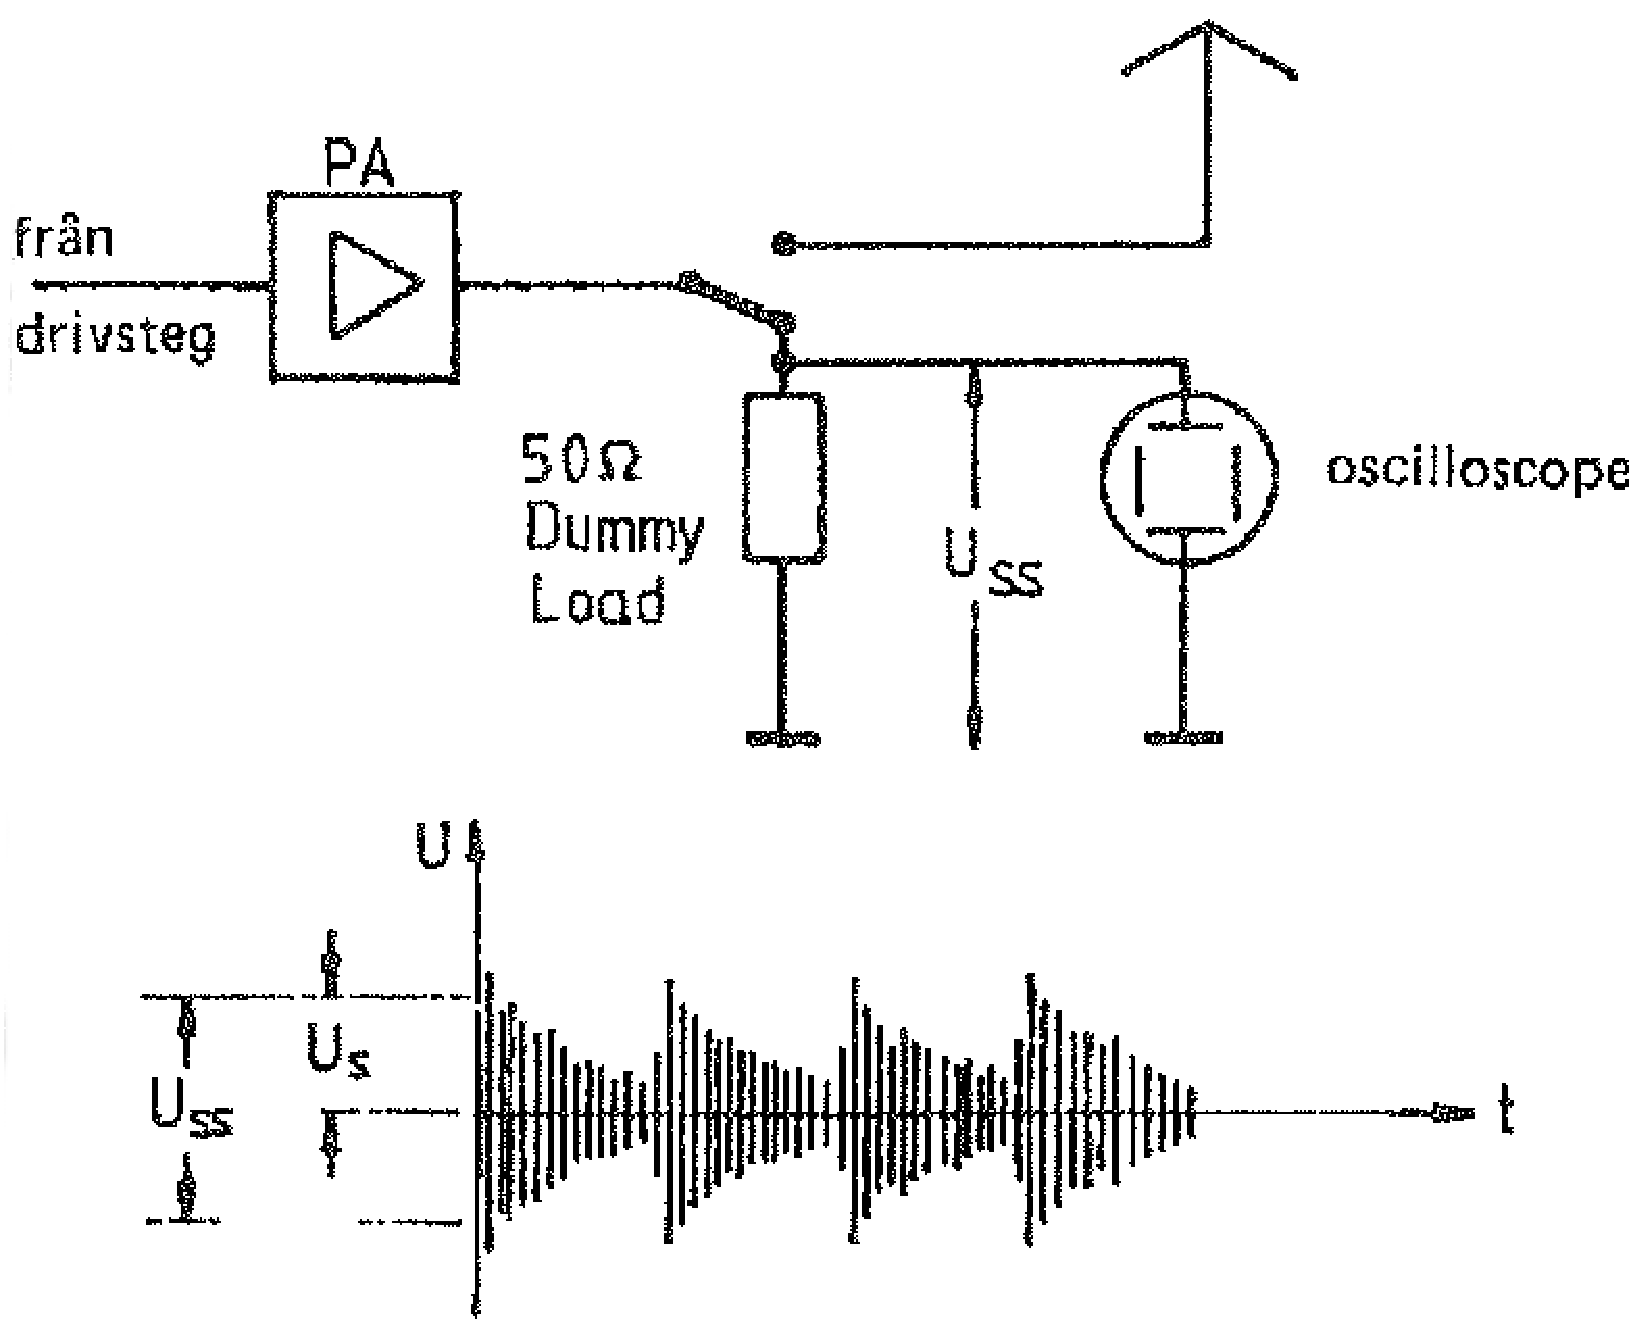
\includegraphics[width=0.5\textwidth]{images/cropped_pdfs/bild_2_3-52.pdf}
	\caption{Bestämning av PEP-effekten}
	\label{fig:BildII3-52}
\end{wrapfigure}

På grund av SSB~signalens karaktär kan man inte mäta effektivvärdet av
uteffekten från en SSB-sändare.

Bild \ref{fig:BildII3-52} visar hur modulationen för ett \emph{aaah} ser ut
på ett oscilloskop.

Moduleringsspänningens topp-topp\-värde \(\hat{u}_{t-t}\) mäts lämpligen med ett
oscilloskop när slutsteget är kopplat till en konstlast.

Med topp-toppvärdet känt kan man med följande formler beräkna
toppvärdet (amplituden)

\(
\begin{array}{lll}
\text{toppvärdet (amplituden)} &  \quad \hat{u}= & \dfrac{\hat{u}_{t-t}}{2}\\
& & \\
\text{effektivvärdet} &\quad  U =& \dfrac{\hat{u}}{\sqrt{2}}
\end{array}
\)

Effekten vid moduleringstopparna, så kallad \emph{Peak Envelope Power (PEP)},
kan beräknas med följande formler.

\(
\begin{array}{ll}
P_{PEP} & = \dfrac{U^2}{R} \text{respektive} \\
&\\
P_{PEP} & = \dfrac{\hat{u}_{t-t}^2}{8R}
\end{array}
\)

\subsection{Linjäritetskontroll vid SSB}
\textbf{HAREC
  b.\ref{HAREC.b.7.2.4}\label{myHAREC.b.7.2.4}
}
\index{SSB!linjäritetskontroll}

\begin{figure}
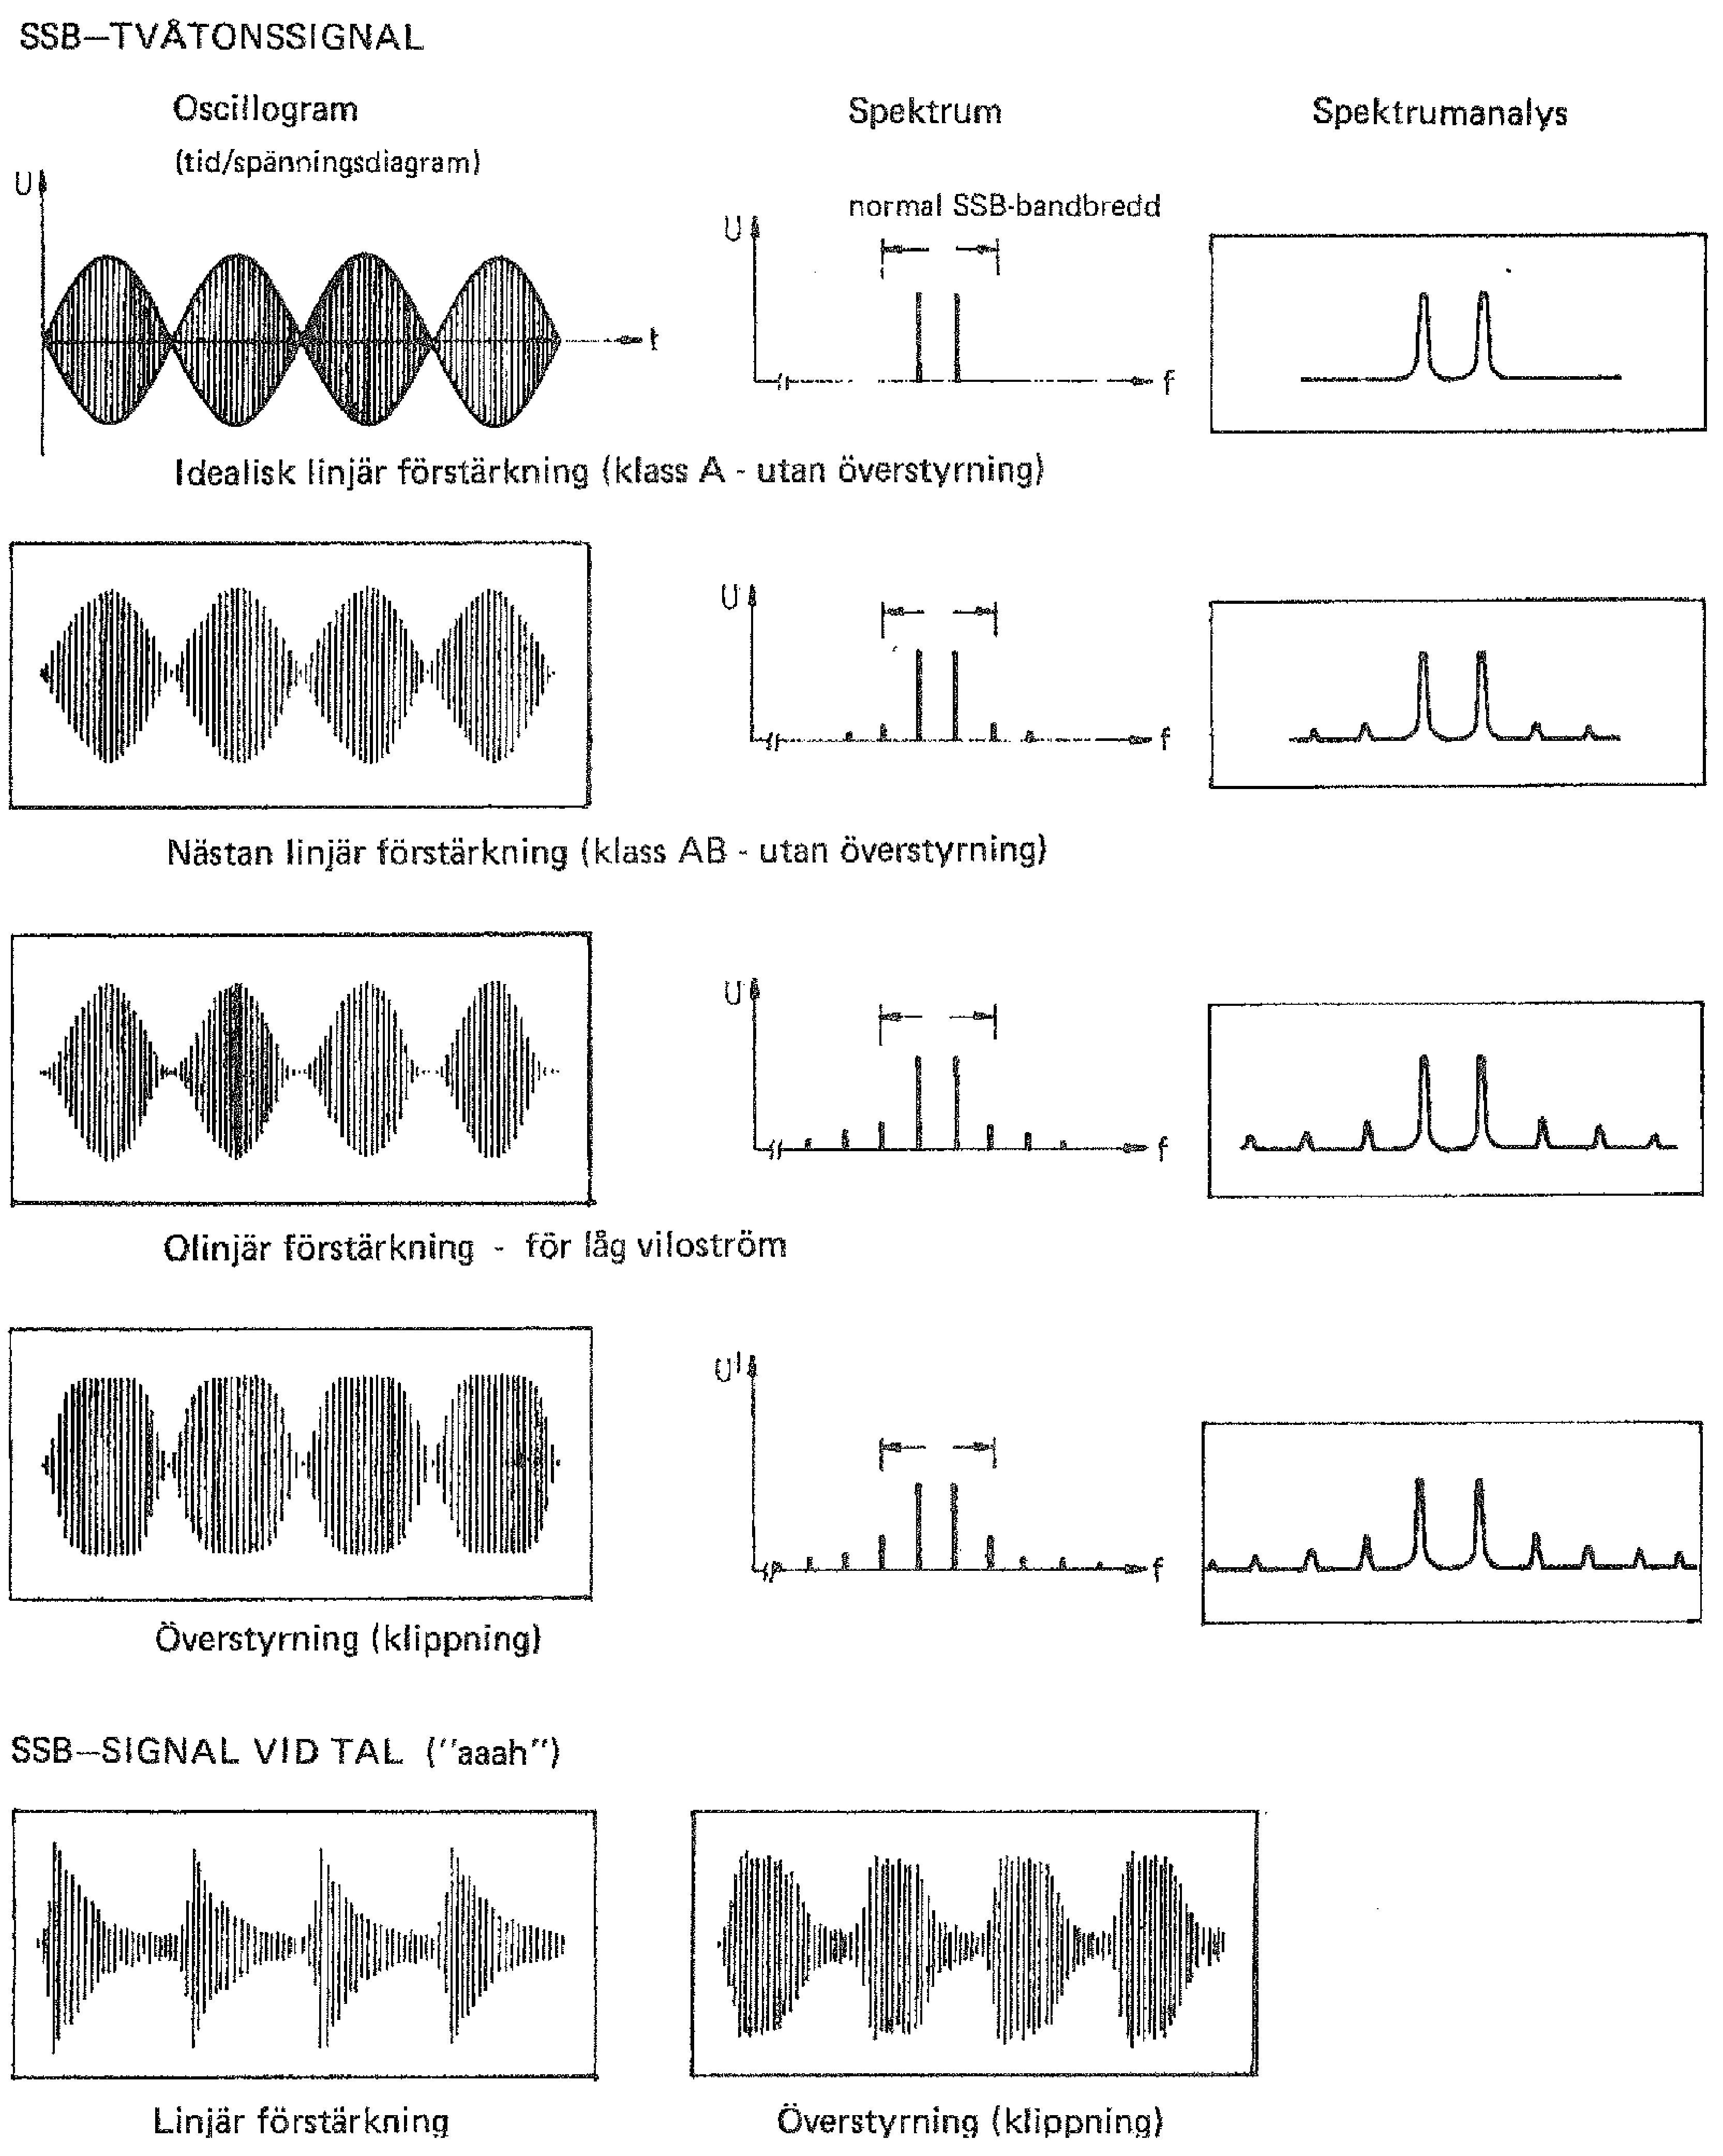
\includegraphics[width=\textwidth]{images/cropped_pdfs/bild_2_3-53.pdf}
\caption{Linjäritetskontroll vid SSB}
\label{fig:BildII3-53}
\end{figure}

Bild \ref{fig:BildII3-53} visar två-tons linjäritetskontroll av SSB.

Linjäriteten i en SSB-sändare kan kontrolleras med ett oscilloskop.
Sändaren moduleras då med två övertonsfria toner.

Slutsteget bör först belastas med konstlast upp till max tillåten effekt.
Resultatet jämförs därefter med antennen som last.

\subsubsection{Linjäritetens betydelse i förstärkare}
\textbf{HAREC a.\ref{HAREC.a.3.4.5}\label{myHAREC.a.3.4.5}}
\index{förstärkning!linjäritet}

\begin{figure}
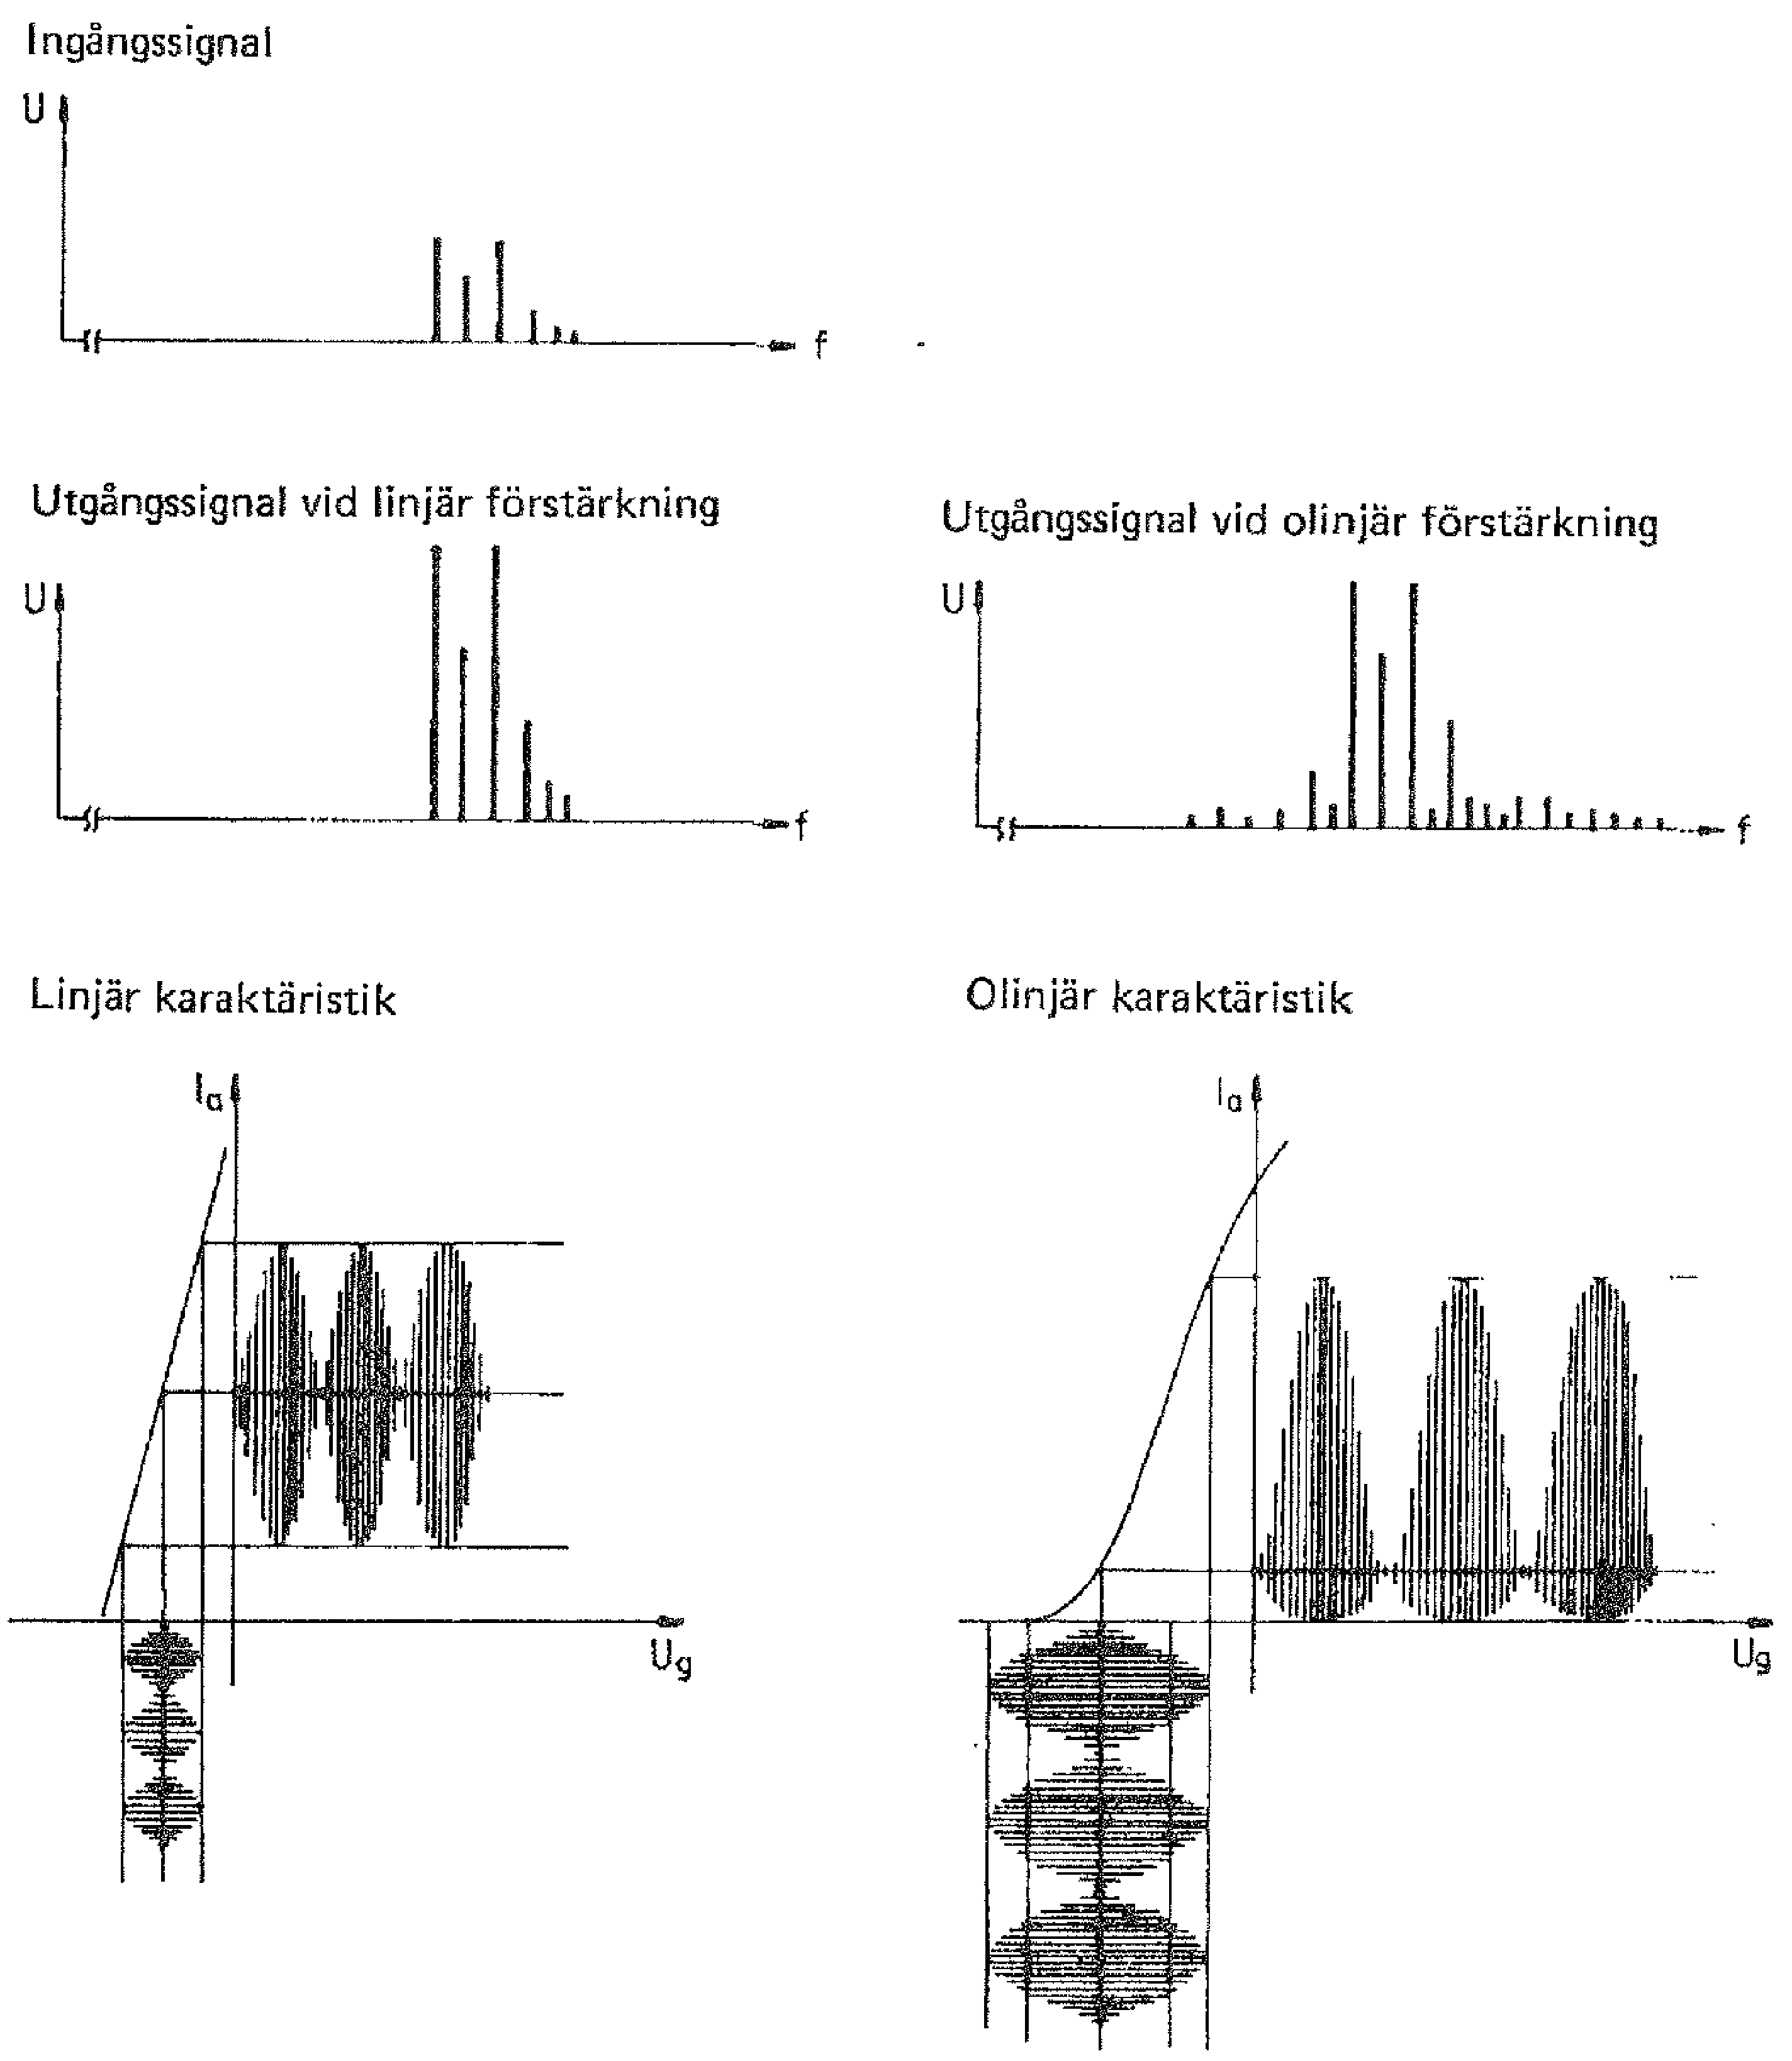
\includegraphics[width=\textwidth]{images/cropped_pdfs/bild_2_3-54.pdf}
\caption{Linjäritetens betydelse}
\label{fig:BildII3-54}
\end{figure}

Bild \ref{fig:BildII3-54} visar mer i detalj olinjäritetens inverkan på
signalen.

Förstärkningen bör ske med god verkningsgrad och minsta möjliga förvrängning,
så att det alstras ett minimum av oönskade frekvenser inom minsta möjliga
bandbredd.

Linjär förstärkning innebär att den är lika över hela det aktuella
frekvensområdet.
Frekvensgången måste därför vara så rak som möjligt.
Med tilltagande olinjäritet tillkommer nämligen allt fler oönskade frekvenser.

Det uppstår blandningsprodukter av högre ordning vid olinjär förstärkning.
Genom förvrängning på grund av olinjär förstärkning uppstår ömsesidiga summa-
och skillnadsfrekvenser av de modulerande frekvenserna.

Varje sådan blandningsprodukt blandar sig additivt och subtraktivt med
grundfrekvenserna till ytterligare blandningsprodukter av näst högre ordning.

Dessa är
\begin{itemize}
\item blandningsprodukter i LF-området och deras övertoner, vilka
  undertrycks i efterföljande HF-krets

\item grundfrekvenserna och deras harmoniska övertoner, som alla ner
  till 1:a harmoniska dämpas kraftigt av efterföljande HF-krets

\item alla summa-och skillnadsfrekvenser av de förstnämnda frekvenserna.
\end{itemize}

I området för nyttofrekvenserna kallas dessa produkter för
intermodulationsprodukter och ger talförvrängning.

Utanför nyttofrekvenserna uppfattas intermodulationsfrekvenserna som
störningar och kallas splatter.
På grund av det lilla frekvensavståndet till nyttosignalen kan den
intermodulation, som alstrats i slutsteget inte filtreras bort i efterhand.

Vid linjär drift uppträder grundfrekvensernas övertoner och
intermodulationsfrekvenser endast svagt inom och utom
överföringsbandet och kommer knappast att uppfattas som inkräktande på
annan radiotrafik.
De svaga övertonerna kommer också att dämpas tillräckligt i \(\pi \)-filtret
och eventuella ytterligare övertonsfilter.


\subsection{Utstyrningskontroll av slutsteg}
\index{förstärkning!utstyrningskontroll}

Slutstegets linjära utstyrningsområde överskrids, om ingångssignalens
amplitud blir för stor.
Då ökar utgångssignalens amplitud inte mycket mer, men utgångssignalens toppar
blir tillplattade (s.k. klippta).
Det betyder att slutsteget är överstyrt.

Vid överstyrning uppstår signalförvrängningar, som medför intermodulation,
förvrängt tal, splatterstörningar och övertoner.
Den extra effektökning som uppnås med överstyrning förbrukas i stort sett
till signalförvrängning och kommer inte nyttosignalen till godo.
Överstyrning ska därför undvikas.

Drivstegets uteffekt får inte vara så stor att slutsteget blir överstyrt.
Ett slutsteg med jordad katod blir fullt utstyrt redan vid en driveffekt av ett
fåtal watt.
Är uteffekten från drivsteget större, än vad som behövs för full utstyrning av
slutsteget, och driveffekten inte kan regleras ner, så måste en dämpsats
kopplas in mellan drivsteg och slutsteg.
En sådan dämpsats kan behöva ta upp en betydande effekt, från en vanligt
förekommande amatörradiosändare med upp till 100~watt PEP.

Ett slutsteg med jordat galler fordrar en större driveffekt, varvid
risken för överstyrning i slutsteget är något mindre och de
förebyggande åtgärderna inte så omfattande.

Linjära slutsteg innehåller oftast en funktion kallad ALC (Automatic Load
Control), som kontinuerligt känner av driveffektens inverkan på slutsteget.
När driveffekten blir för hög, alstras en kontrollspänning i proportion till
utstyrningsgraden.
ALC-spänning återförs till drivsteget och reglerar dess uteffekt så att
överstyrning av slutsteget inte sker.
I transistoriserade slutsteg skapas ALC-spänningen genom likriktning av
slutstegets utspänning.
I rörslutsteg börjar styrgallret dra ström, när styrgallerspänningen
blir positiv i signaltopparna, vilket används för att styra ALC-spänningen.
När ALC-regleringen sätter in, är överstyrningen således redan ett faktum.
Överstyrning kan ske både på LF- och HF-nivå.

En orsak till övermodulering är för stor amplitud på den modulerande signalen.
Detta kan bland annat avhjälpas med inställning av mikrofonförstärkaren och
riktig mikrofonhantering.
